% !TEX program = xelatex

\documentclass[12pt,a4paper]{article}
\usepackage[UTF8]{ctex}
\usepackage{float}
\usepackage{amsmath}
\usepackage{amsfonts}
\usepackage{enumerate}
\usepackage{booktabs}
\usepackage{graphicx}
\usepackage{longtable}
\usepackage{subfigure}

\usepackage{url}
\usepackage{multirow}

% for plotting 
\usepackage{caption}
\usepackage{pgfplots}

% for pseudo code 
\usepackage{algorithm}
\usepackage[noend]{algpseudocode}

% for reference 
\usepackage{hyperref}
\usepackage{cleveref}

% for code 
\usepackage{listings}
\usepackage{xcolor}
\usepackage{fontspec}
\definecolor{darkgreen}{rgb}{0,0.6,0}
\newfontfamily\consolas{Consolas}

\lstset {
    basicstyle=\footnotesize\consolas, % basic font setting
    breaklines=true, 
    frame=single,     % {single, shadowbox, bottomline}
    keywordstyle=\color{blue}, 
    commentstyle=\color{darkgreen},
    stringstyle=\color{red},
    showstringspaces=false,
    % backgroundcolor=\color{black!5}, % set backgroundcolor
    numbers=left, 
    numberstyle=\ttfamily,
}

% Microsoft Word A4 paper default layout 
\usepackage[a4paper, left=3.18cm, right=3.18cm, top=2.54cm, bottom=2.54cm]{geometry}

% \captionsetup[figure]{labelfont={bf}, name={Figure}}
% \captionsetup[table]{labelfont={bf}, name={Table}}

\crefname{equation}{方程}{方程}
\Crefname{equation}{方程}{方程}
\crefname{table}{表}{表}
\Crefname{table}{表}{表}
\crefname{figure}{图}{图}
\Crefname{figure}{图}{图}

\title{数学实验:第四次作业}
\author{计算机系 \quad 计73 \quad 2017011620 \quad 李家昊}
\date{\today}

% 实验报告格式的基本要求

% 系别、班级、学号、姓名

% 1 实验目的
% 2 题目
%   2.1 计算题:题号,算法设计(包括计算公式),程序,计算结果(计算机输出),结果分析,结论。
%   2.2 应用题:题号,问题分析,模型假设,模型建立,算法设计(包括计算公式),程序,计算结果(计算机输出),结果的数学分析,结果的实际意义,结论。
% 3 收获与建议

% Calc
% \subsubsection{算法设计}
% \subsubsection{Matlab程序}
% \subsubsection{计算结果}
% \subsubsection{结果分析}
% \subsubsection{结论}

% App
% \subsubsection{问题分析}
% \subsubsection{模型假设}
% \subsubsection{模型建立}
% \subsubsection{算法设计}
% \subsubsection{Matlab程序}
% \subsubsection{计算结果}
% \subsubsection{结果的数学分析}
% \subsubsection{结果的实际意义}
% \subsubsection{结论}

\begin{document}

\maketitle

\section{实验目的}

\begin{itemize}
    \item 掌握用MATLAB软件求解非线性方程和方程组的基本方法,并对结果作初步分析。
    \item 练习用非线性方程和方程组建立实际问题的模型并进行求解。
\end{itemize}

\section{问题求解}

\subsection{Chap6-Ex3 利率(应用题)}

\subsubsection{问题分析}

题目给出了按揭贷款的本金总额,还款期数,以及每期还款金额,需要求出贷款利率,这是一个非线性方程求解问题。

\subsubsection{模型假设}

考虑到实际情况,该模型基于以下假设,
\begin{enumerate}
    \item 借款人能够按时按量还款。
    \item 偿还过程中本金利率不变。
\end{enumerate}

\subsubsection{模型建立}

\paragraph{数学模型} 设贷款总额为$Q$,每期贷款利率为$x>0$,第$n$期还款后剩余本金为$a_n$,每期还款金额为$q$,共分$N$期还清,则序列$\{a_n\}$满足差分方程,
\begin{equation}
    a_{n+1} = (1+x)a_{n} - q, \quad n = 0,1,2,\cdots,N-1
\end{equation}
可解得其通项为,
\begin{equation}\label{eq:ex3_difference}
    a_{n} = (1+x)^n \left(a_0 - \frac{q}{x}\right) + \frac{q}{x}, \quad n = 0,1,2,\cdots,N
\end{equation}
由条件,有$a_0 = Q$,$a_N=0$,带入$n=N$到\Cref{eq:ex3_difference},得到,
\begin{equation}
    0 = (1+x)^N \left(Q - \frac{q}{x}\right) + \frac{q}{x}
\end{equation}
进一步化简得,
\begin{equation}\label{eq:ex3_model}
    N \ln (1+x) + \ln \left(1-\frac{Q}{q} x\right) = 0, \quad x \in \left(0, \frac{q}{Q}\right)
\end{equation}
记\Cref{eq:ex3_model}左端为$f(x)$,则有$f(x)=0$,即为本题的模型。

\paragraph{零点分析} 那么,$f(x)$有没有零点呢?如果有,则有多少个零点?为了进一步研究$f(x)$的零点,这里首先求出它的导函数,
\begin{equation}
    f'(x) = \frac{(Nq - Q) - (N+1)Qx}{(1+x)(q-Qx)}
\end{equation}
令$f'(x) = 0$,解得,
\begin{equation}
    x_1 = \frac{Nq - Q}{(N+1)Q}
\end{equation}
由于利率的存在,总还款金额必定大于贷款总额,即$Nq > Q$,因此$0 < x_1 < q/Q$,且由于$0 < x < q/Q$,因此$q-Qx>0$。

由此可得,当$x \in (0, x_1)$时,$f'(x)>0$,$f(x)$递增;当$x\in (x_1, q/Q)$时,$f'(x)<0$,$f(x)$递减。

由于$f(0) = 0$,因此$f(x_1) > 0$,由于$\lim_{x\rightarrow q/Q^-} f(x)= -\infty$,且$f(x)$连续,由零点定理知,$f(x)$在区间$(x_1, q/Q)$中必有一个零点,由上文分析的$f(x)$的单调性可知,该零点为$f(x)$的唯一零点。

\subsubsection{算法设计}

首先应当画出$f(x)$在$x\in (0, q/Q)$的图像,确定函数零点的大致位置,将其作为初值。由$f(x)$的单调性可知零点两侧异号,因此可利用\texttt{fzero}命令求解。

\subsubsection{Matlab程序}

请参见附录\ref{sec:ex3_code}。

\subsubsection{计算结果}

\paragraph{第一小问} 由题意,此处贷款月利率为$x$,应还款总额$Q=15$万元,每月还款$q=0.1$万元,分$N=180$个月还清,带入\Cref{eq:ex3_model}中,得到,
\begin{equation}
    f(x) = 180 \ln (1+x) + \ln (1-150x)
\end{equation}

画出$f(x)$的图像,如\Cref{fig:ex3_1_graph}所示,可见$f(x)$的唯一零点在0.002附近,将其作为初值,用\texttt{fzero}求解得到结果为$\hat{x}=0.2081\%$,其对应的绝对误差为$e=f(\hat{x})=-3.1086\times 10^{-15}$。

\begin{figure}[t]
    \centering
    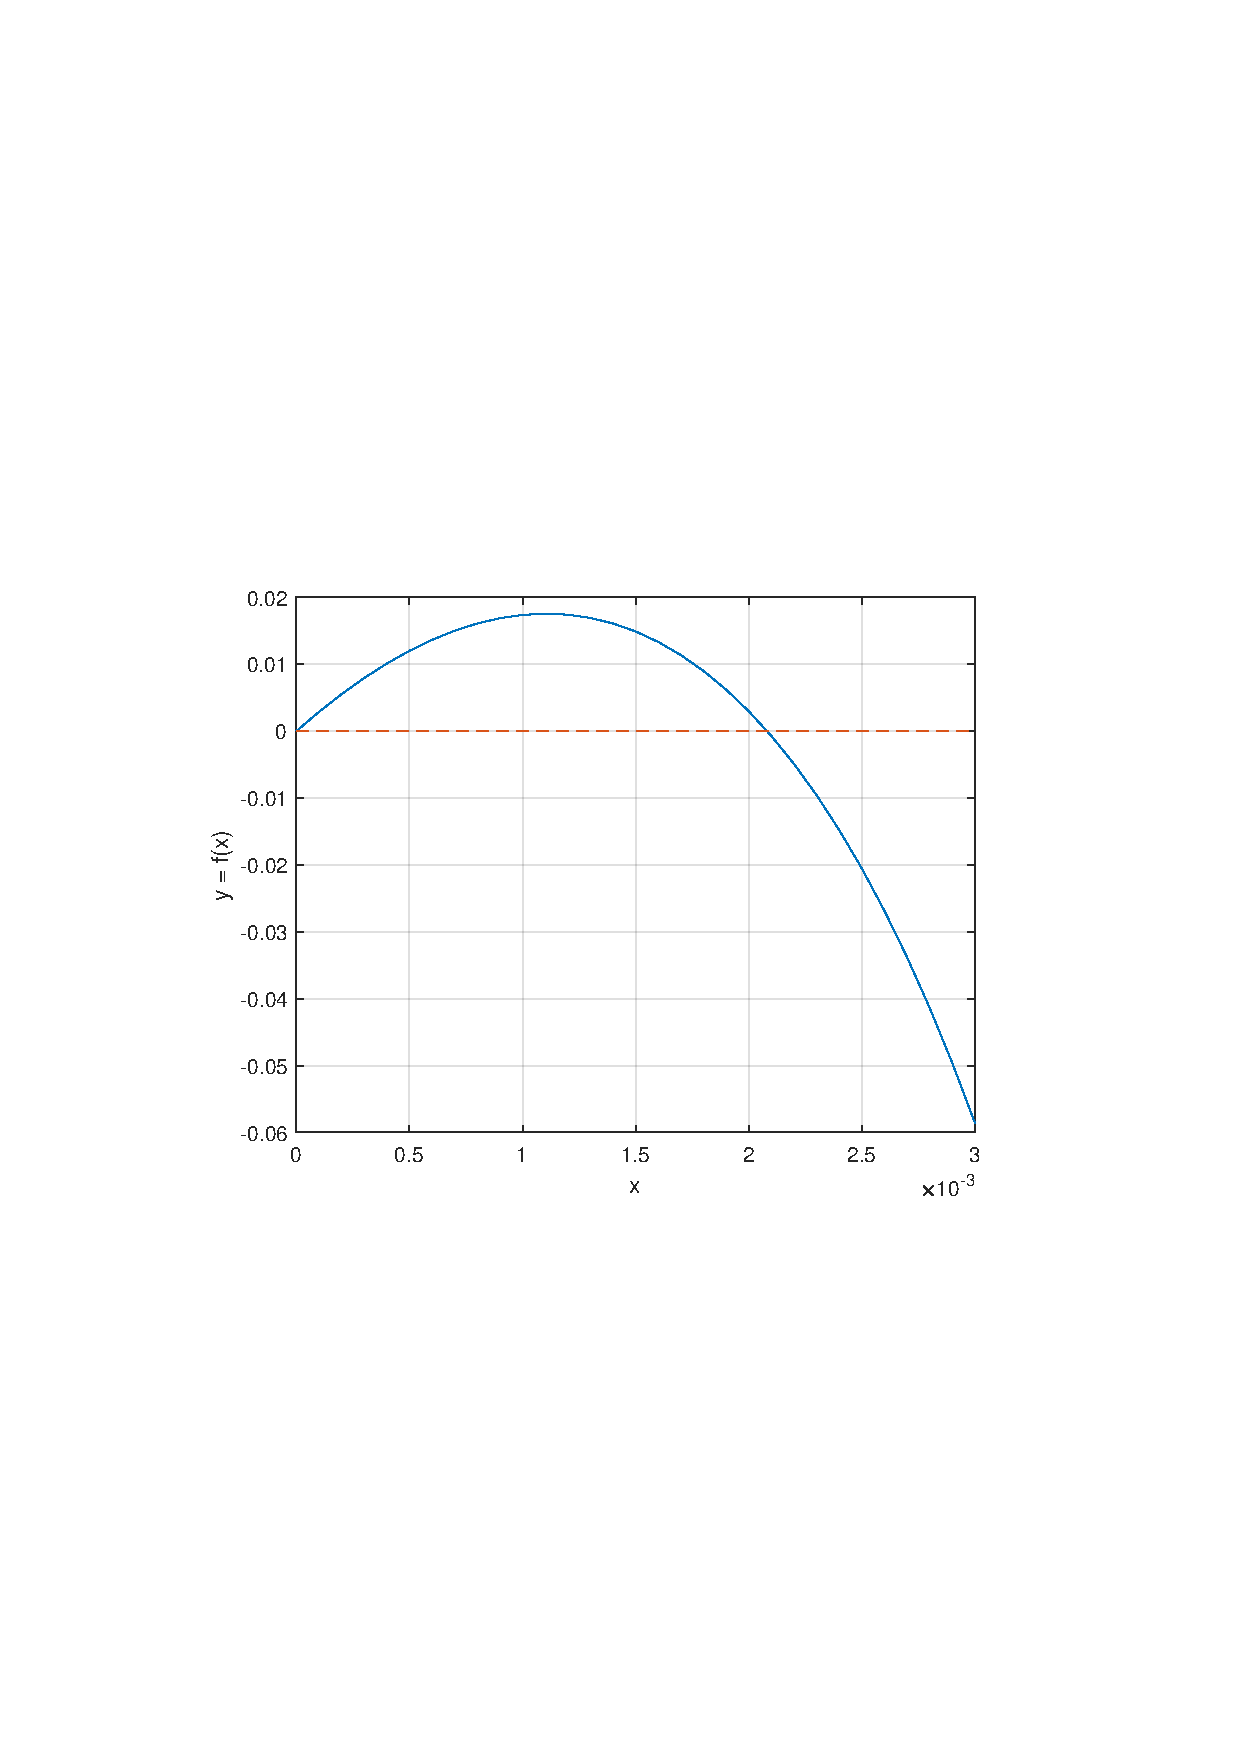
\includegraphics[width=0.8\textwidth,trim={3.09cm 9.295cm 3.09cm 9.295cm},clip]{fig/ex3_1_graph.pdf}
    \caption{$f(x)$在零点附近的图像}
    \label{fig:ex3_1_graph}
\end{figure}

\paragraph{第二小问} 按月还款时,贷款月利率为$x$,应还款总额$Q=50$万元,每月还款$q=0.45$万元,分$N=180$个月还清,带入\Cref{eq:ex3_model}中,得到,
\begin{equation}
    f(x) = 180 \ln (1+x) + \ln \left(1-\frac{1000}{9}x\right)
\end{equation}

画出$f(x)$的图像,如\Cref{fig:ex3_2_graph}所示,可见$f(x)$的唯一零点在0.006附近,将其作为初值,用\texttt{fzero}求解得到结果为$\hat{x}=0.5851\%$,其对应的绝对误差为$e=f(\hat{x})=-1.7542\times 10^{-14}$。

\begin{figure}[t]
    \centering
    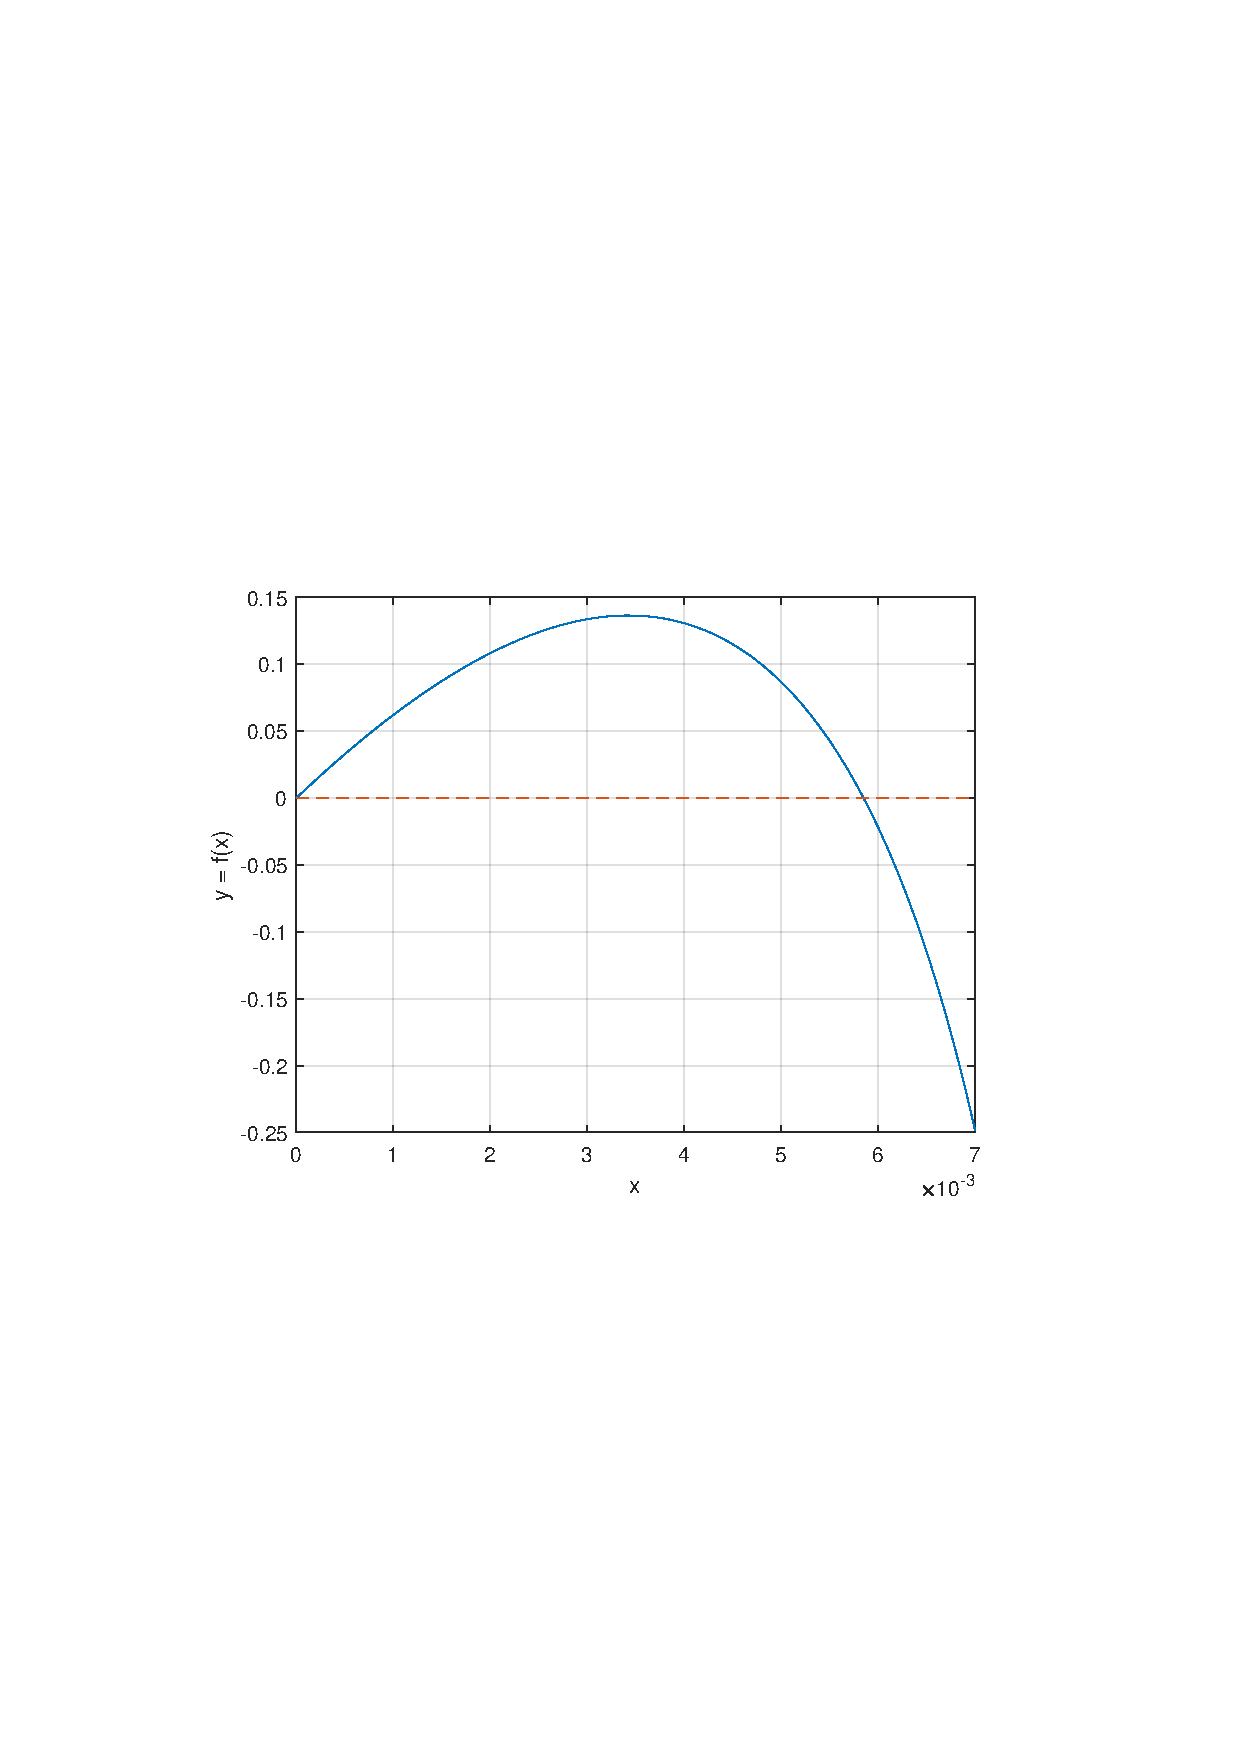
\includegraphics[width=0.8\textwidth,trim={3.09cm 9.295cm 3.09cm 9.295cm},clip]{fig/ex3_2_graph.pdf}
    \caption{$f(x)$在零点附近的图像}
    \label{fig:ex3_2_graph}
\end{figure}

按年还款时,贷款年利率为$x$,应还款总额$Q=50$万元,每年还款$q=4.5$万元,分$N=20$年还清,带入\Cref{eq:ex3_model}中,得到,
\begin{equation}
    f(x) = 20 \ln (1+x) + \ln \left(1-\frac{100}{9}x\right)
\end{equation}

画出$f(x)$的图像,如\Cref{fig:ex3_3_graph}所示,可见$f(x)$的唯一零点在0.065附近,将其作为初值,用\texttt{fzero}求解得到结果为$\hat{x}=6.3949\%$,其对应的绝对误差为$e=f(\hat{x})=-4.4409\times 10^{-15}$。

\begin{figure}[t]
    \centering
    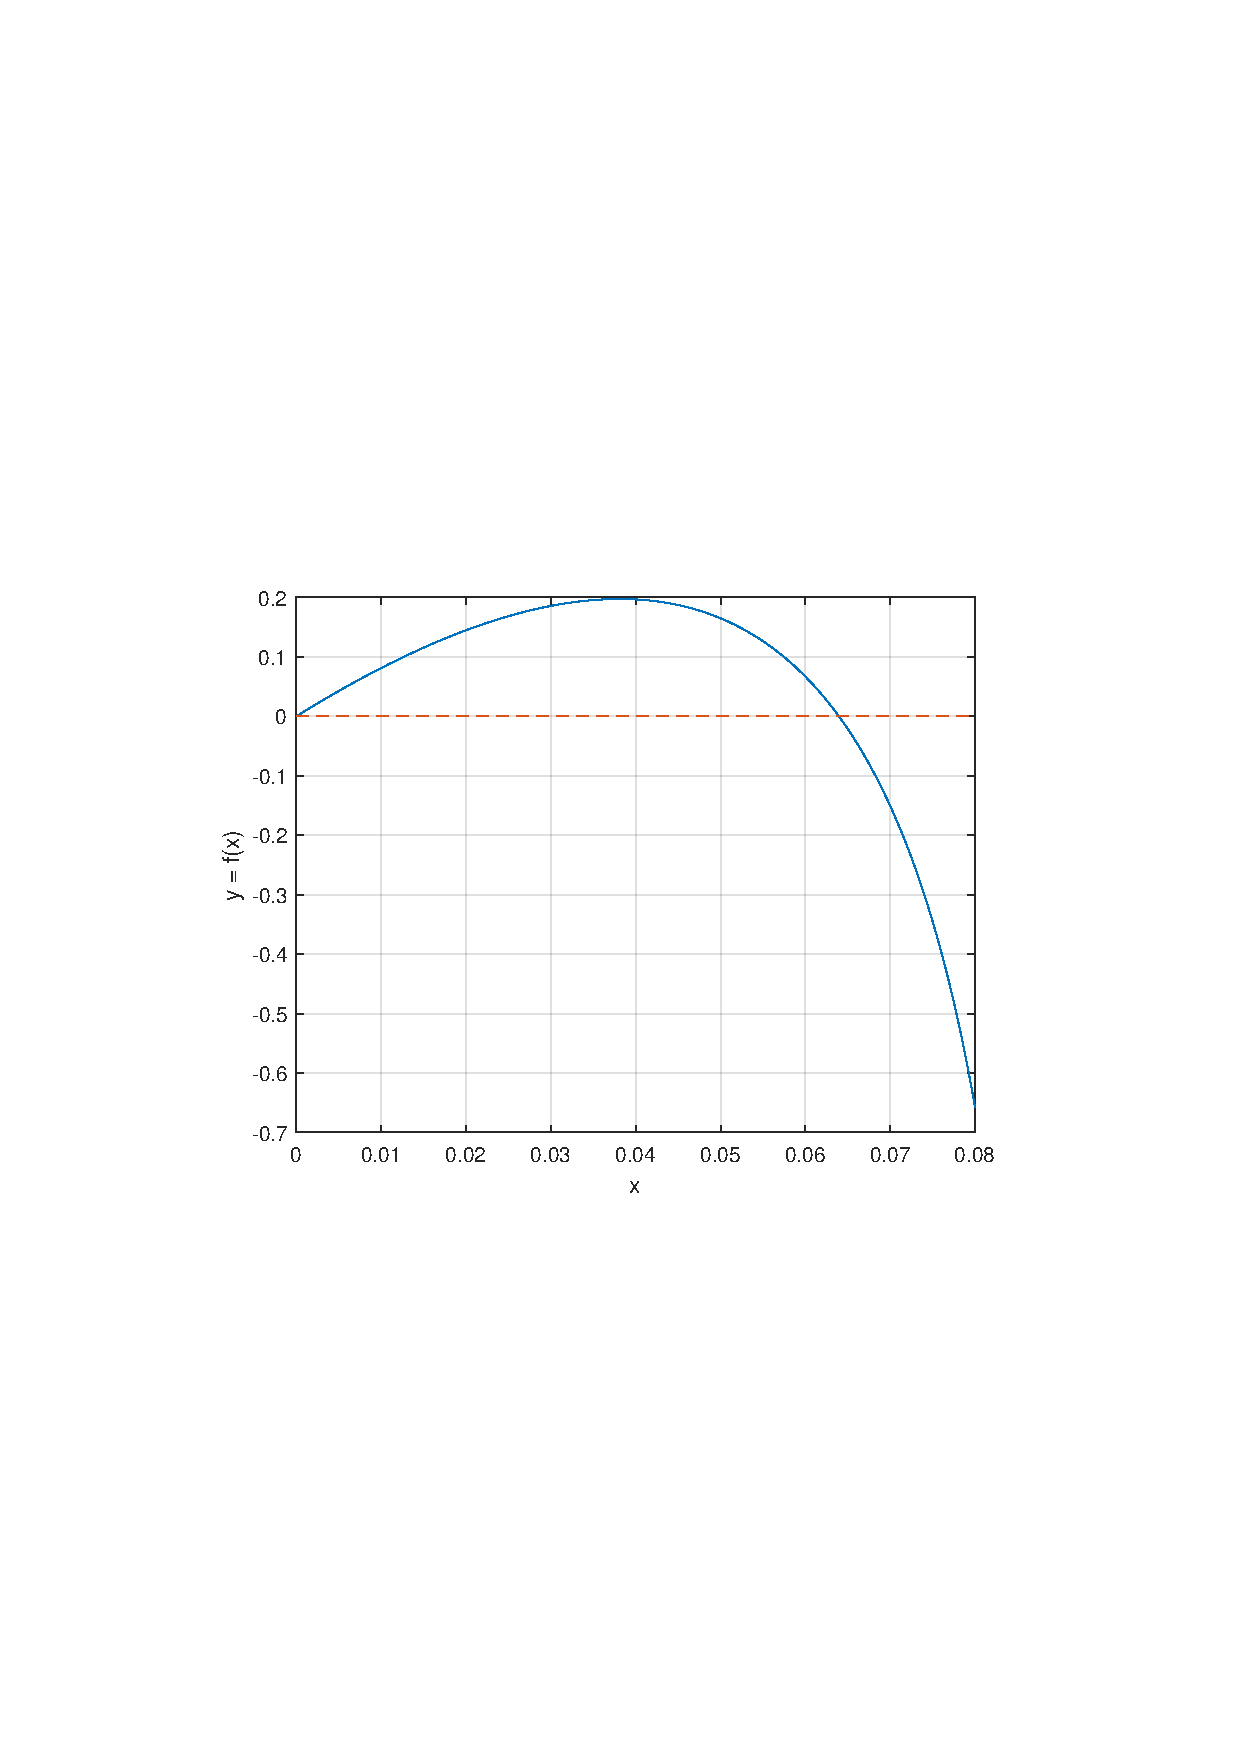
\includegraphics[width=0.8\textwidth,trim={3.09cm 9.295cm 3.09cm 9.295cm},clip]{fig/ex3_3_graph.pdf}
    \caption{$f(x)$在零点附近的图像}
    \label{fig:ex3_3_graph}
\end{figure}

\subsubsection{结果的数学分析}

在三个方程中,方程的绝对误差均控制在$10^{-13}$以内,十分精确,具有实际参考价值。

\subsubsection{结果的实际意义}

对于第二小问,第一家银行的贷款月利率为0.5851\%,第二家银行的贷款年利率为6.3949\%,按照年利率等于12倍月利率计算,则第二家银行的贷款月利率为0.5329\%,比第一家银行的月利率更低,因此,从利率角度看,第二家银行更优惠。

如果从还款总额来看,第一家银行的还款总额为81万,第二家银行的还款总额为90万,若不考虑通货膨胀等因素,第一家银行将比第二家银行更优惠。因此,在向银行贷款时,应当综合多方面因素考虑其贷款政策,做出合理的决定。

本题根据按揭贷款的本金总额,还款期数,以及每期还款金额,求出了贷款利率,该结果具有一定的参考价值。然而,在现实生活中,通常是给定本金总额,还款期数,以及贷款基准利率,求每期还款金额,这往往是借款人和贷款机构最关心的事情。

\subsubsection{结论}

小张夫妇的贷款月利率为0.2081\%。从利率角度看,第二家银行更优惠。

\subsection{Chap6-Ex6 均相共沸混合物(应用题)}

\subsubsection{问题分析}

题目给定四种物质对应的参数和相互作用矩阵,需要求出给定压强下的共沸混合物的温度和组分,这是一个非线性方程组求解问题。

\subsubsection{模型假设}

考虑到实际情况,模型的建立基于以下假设,
\begin{enumerate}
    \item 给定的物质能混合共存,不发生相互化学作用。
    \item 均相共沸混合物满足稳定条件。
\end{enumerate}

\subsubsection{模型建立}

设该混合物由$n$个组分组成,组分$i$所占比例为$x_i\ (i=1,2,\cdots,n)$,则有,
\begin{equation}\label{eq:ex6_component}
    \sum_{i=1}^n x_i = 1, \quad x_i \ge 0
\end{equation}
由假设2,均相共沸混合物应该满足稳定条件,在压强$P$不大时,该条件可以表示为,
\begin{equation}\label{eq:ex6_pressure}
    P = \gamma_i P_i, \quad i=1,2,\cdots,n
\end{equation}
其中$P_i$为组分$i$的饱和汽相压强,$\gamma_i$为组分$i$的液相活度系数。$P_i$可根据下式确定,
\begin{equation}\label{eq:ex6_log_pressure}
    \ln P_i = a_i - \frac{b_i}{T + c_i}, \quad i = 1,2,\cdots,n
\end{equation}
其中$a_i,b_i,c_i$为常数,$T$为温度。$\gamma_i$可根据下式确定,
\begin{equation}\label{eq:ex6_log_gamma}
    \ln \gamma_i = 1 - \ln\left(\sum_{j=1}^n x_j q_{ij}\right) - \sum_{j=1}^n\left(\frac{x_j q_{ji}}{\sum_{k=1}^n x_k q_{jk}}\right),\quad i=1,2,\cdots,n
\end{equation}
其中$q_{ij}$表示组分$i$与组分$j$的交互作用参数,$q_{ij}$组成交互作用矩阵$Q$。将\Cref{eq:ex6_pressure}两边取对数后,将\Cref{eq:ex6_log_pressure},\Cref{eq:ex6_log_gamma}带入其中,考虑到只有组分$i$参与到共沸混合物时才满足上述条件,因此需要添加一个组分因子$x_i$,得到,
\begin{equation}\label{eq:ex6_system}
    x_i\left[1 - \ln\left(\sum_{j=1}^n x_j q_{ij}\right) - \sum_{j=1}^n\left(\frac{x_j q_{ji}}{\sum_{k=1}^n x_k q_{jk}}\right) + a_i - \frac{b_i}{T + c_i} - \ln P\right] = 0
\end{equation}
其中$i=1,2,\cdots,n$。

\Cref{eq:ex6_component}和\Cref{eq:ex6_system}共有$n+1$个方程,其中含$n+1$个变量,组成了一个非线性方程组,构成了此题的模型。

\subsubsection{算法设计}

在实际求解过程中,首先利用\Cref{eq:ex6_component}消去其中一个变量,即,
\begin{equation}
    x_n = 1 - \sum_{i=1}^{n-1} x_i
\end{equation}
并将其带入\Cref{eq:ex6_system}中,得到含有$n$个变量的$n$个非线性方程,利用Matlab优化工具箱的\texttt{fsolve}命令即可求出该非线性方程组的解,需要注意的是,在不同初值条件下方程可能有不同的解,因此需要对初值进行搜索和试探。

对于误差分析,记所求的方程组为$\boldsymbol{f}(\boldsymbol{x}) = \boldsymbol{0}$,其中$\boldsymbol{f} = (f_1, f_2, \cdots f_n)$代表$n$个方程对应的函数,$\boldsymbol{x}=(x_1,\cdots, x_{n-1}, T)$为$n$个未知数,设求出的一组解为$\hat{\boldsymbol{x}}$,则定义方程的绝对误差为$\boldsymbol{e} = \boldsymbol{f}(\hat{\boldsymbol{x}})$,通过计算误差的p-范数,可以大致了解方程解的精确程度。

\subsubsection{Matlab程序}

请参见附录\ref{sec:ex6_code}。

\subsubsection{计算结果}

设置四重循环搜索初值条件,第一重遍历$x_1 \in \{0.0, 0.1, \cdots, 1.0\}$,第二重遍历$x_2 \in \{0.0, 0.1, \cdots, 1-x_1\}$,第三重遍历$x_3 \in \{0.0, 0.1, \cdots, 1-x_1-x_2\}$,第四重遍历$T \in \{0, 10, \cdots, 100\}$,对于给定的一组初值$(x_1, x_2, x_3, T)$,求解非线性方程组。

经过初值搜索,一共得到3025组解,其中大部分是重复解,经过去重并过滤掉不合法的解后,合法的方程解如\Cref{tab:ex6_all_solutions}所示。

根据题意,需要形成共沸混合物,其中至少有两种物质的组分,因此需要进一步过滤掉仅含有一种组分的方程解,得到最终可能的共沸混合物组分及温度,共有三种情况,列举如下,
\begin{enumerate}
    \item $x_1 = 62.47\%, \quad x_2 = 37.53\%, \quad x_3 = 0.00\%, \quad x_4 = 0.00\%, \quad T = 58.1358$
    \item $x_1 = 0.00\%, \quad x_2 = 58.58\%, \quad x_3 = 41.42\%, \quad x_4 = 0.00\%, \quad T = 71.9657$
    \item $x_1 = 0.00\%, \quad x_2 = 78.03\%, \quad x_3 = 0.00\%, \quad x_4 = 21.97\%, \quad T = 76.9613$
\end{enumerate}

\begin{table}
    \centering
    \caption{不同初值条件下求出的混合物组分和温度,以及方程的绝对误差($\times 10^{-5}$)}
    \label{tab:ex6_all_solutions}
    \begin{tabular}{c|ccccc|ccc}
        \toprule
        No. & \(x_1\) & \(x_2\) & \(x_3\) & \(x_4\) & \(T\) &
        \(||\boldsymbol{e}||_1\) & \(||\boldsymbol{e}||_2\) &
        \(||\boldsymbol{e}||_\infty\)\tabularnewline
        \midrule
        1 & 0.6247 & 0.3753 & 0.0000 & 0.0000 & 58.1358 & 0.0000 & 0.0000 &
        0.0000\tabularnewline
        2 & 0.0000 & 0.5858 & 0.4142 & 0.0000 & 71.9657 & 0.0265 & 0.0160 &
        0.0111\tabularnewline
        3 & 0.0000 & 0.0000 & 1.0000 & 0.0000 & 82.5567 & 0.0005 & 0.0003 &
        0.0002\tabularnewline
        4 & 0.0000 & 0.0000 & 0.0000 & 1.0000 & 97.7712 & 0.0000 & 0.0000 &
        0.0000\tabularnewline
        5 & 0.0000 & 0.7803 & 0.0000 & 0.2197 & 76.9613 & 0.0001 & 0.0001 &
        0.0000\tabularnewline
        6 & 0.0000 & 1.0000 & 0.0000 & 0.0000 & 80.1162 & 0.0000 & 0.0000 &
        0.0000\tabularnewline
        7 & 0.0000 & 0.0000 & 0.0000 & 1.0000 & 97.7711 & 0.4756 & 0.4365 &
        0.4356\tabularnewline
        8 & 1.0000 & 0.0000 & 0.0000 & 0.0000 & 64.5465 & 0.0001 & 0.0001 &
        0.0001\tabularnewline
        9 & 0.0000 & 0.0000 & 0.0000 & 1.0000 & 97.7709 & 1.1153 & 0.9356 &
        0.9283\tabularnewline
        \bottomrule
    \end{tabular}
\end{table}

\subsubsection{结果的数学分析}

由\Cref{tab:ex6_all_solutions}可以看出,方程解的误差的1-范数,2-范数,以及$\infty$-范数均控制在$10^{-4}$以内,最终选取的三组解的误差控制在$10^{-6}$以内,因此方程的解较为精确,最终结果可作为实际应用的参考。

\subsubsection{结果的实际意义}

在压强为$760\ \mathrm{mmHg}$下,为了形成均相共沸混合物,计算机给出了三组可能的组分和温度结果,三组结果都十分精确地满足了稳定性条件,具有实际参考价值。在此基础上,需要进一步通过实验验证其可行性,该理论计算的结果对实际实验具有重要的指导意义。

\subsubsection{结论}

在压强为$760\ \mathrm{mmHg}$下,为了形成均相共沸混合物,温度和组分有三种可能的情况,分别为,
\begin{enumerate}
    \item 温度为58.1358度,组分1占62.47\%,组分2占37.53\%,无其余组分。
    \item 温度为71.9657度,组分2占58.58\%,组分3占41.42\%,无其余组分。
    \item 温度为76.9613度,组分2占78.03\%,组分4占21.97\%,无其余组分。
\end{enumerate}

\subsection{Chap6-Ex8 价格混沌(计算题)}

\subsubsection{算法设计}

由题意,商品在$t$时期的市场价格为$p_t$,需求函数为$D(p_t) = c-d p_t,\ (c,d>0)$,生产方期望价格为$q_t$,供应函数为$S(q_t)$,供销平衡时$S(q_t) = D(p_t)$。生产方在$t+1$时期会将价格调整为$q_{t+1}$,其中$q_{t+1}-q_t=r[p(t)-q(t)],\ (0<r<1)$。设$S(x) = \arctan(\mu x), \mu = 0.8, d = 0.25, r = 0.3$,以$c$为可变参数。

由上述条件,可得出$q_t$的差分方程为,
\begin{equation}\label{eq:ex8_model}
    q_{t+1} = \frac{r}{d}\left[c - \arctan(\mu q_t)\right] + (1-r)q_t
\end{equation}

为了观察其分岔与混沌现象,设置参数集$\mathcal{C}=\{c_i\}_{i=1}^{m}$,其中$c_i$按大小排序,在每个固定的参数$c_i\in\mathcal{C}$下,迭代$n$次计算序列$q_t$,并画出序列的第$n_s$到第$n$个点。

为了找到具体的分岔点数值,观察到当$t$充分大时,分岔序列$q_t$是周期性的,且周期恰为分岔数,因此,首先在每个参数$c_i$下,求出当$t$充分大时$q_t$的周期$T_i$,其中$T$必然为2的某个幂,然后遍历每个参数$c_i$,若其对应$q_t$的周期$T_i=2T_{i-1}$,则$c_i$即为一个分岔点。

\subsubsection{Matlab程序}

请参见附录\ref{sec:ex8_code}。

\subsubsection{计算结果}

当参数$c$在$[-2, 2]$区间内变化时,生产方期望价格会出现分岔与混沌现象,如\Cref{fig:ex8_chaos}所示。由于题目说明$c>0$,因此这里只关心$c>0$的情况,即从右向左寻找分岔点。

前四个分岔点位置附近的图像如\Cref{fig:ex8_forks}所示,后续的分岔点不一一画出,具体数值如\Cref{tab:ex8_forks}所示,表格中列出了前六个分岔点,其中$c_n$为第$n$个分岔点对应的参数$c$的值,根据这些分岔点$c_n$,可计算出其差值比$\dfrac{c_n-c_{n-1}}{c_{n+1}-c_n}$,同样列在了表格中。

为了讨论价格$q_t$的变化规律,这里根据分岔点的位置选取了6个参数$c$值,分别对应着1分岔,2分岔,4分岔,8分岔,16分岔,以及32分岔,在每个$c$值下对应的$q_t$随$t$变化的图像如\Cref{fig:ex8_q_t}所示。

\begin{figure}[t]
    \centering
    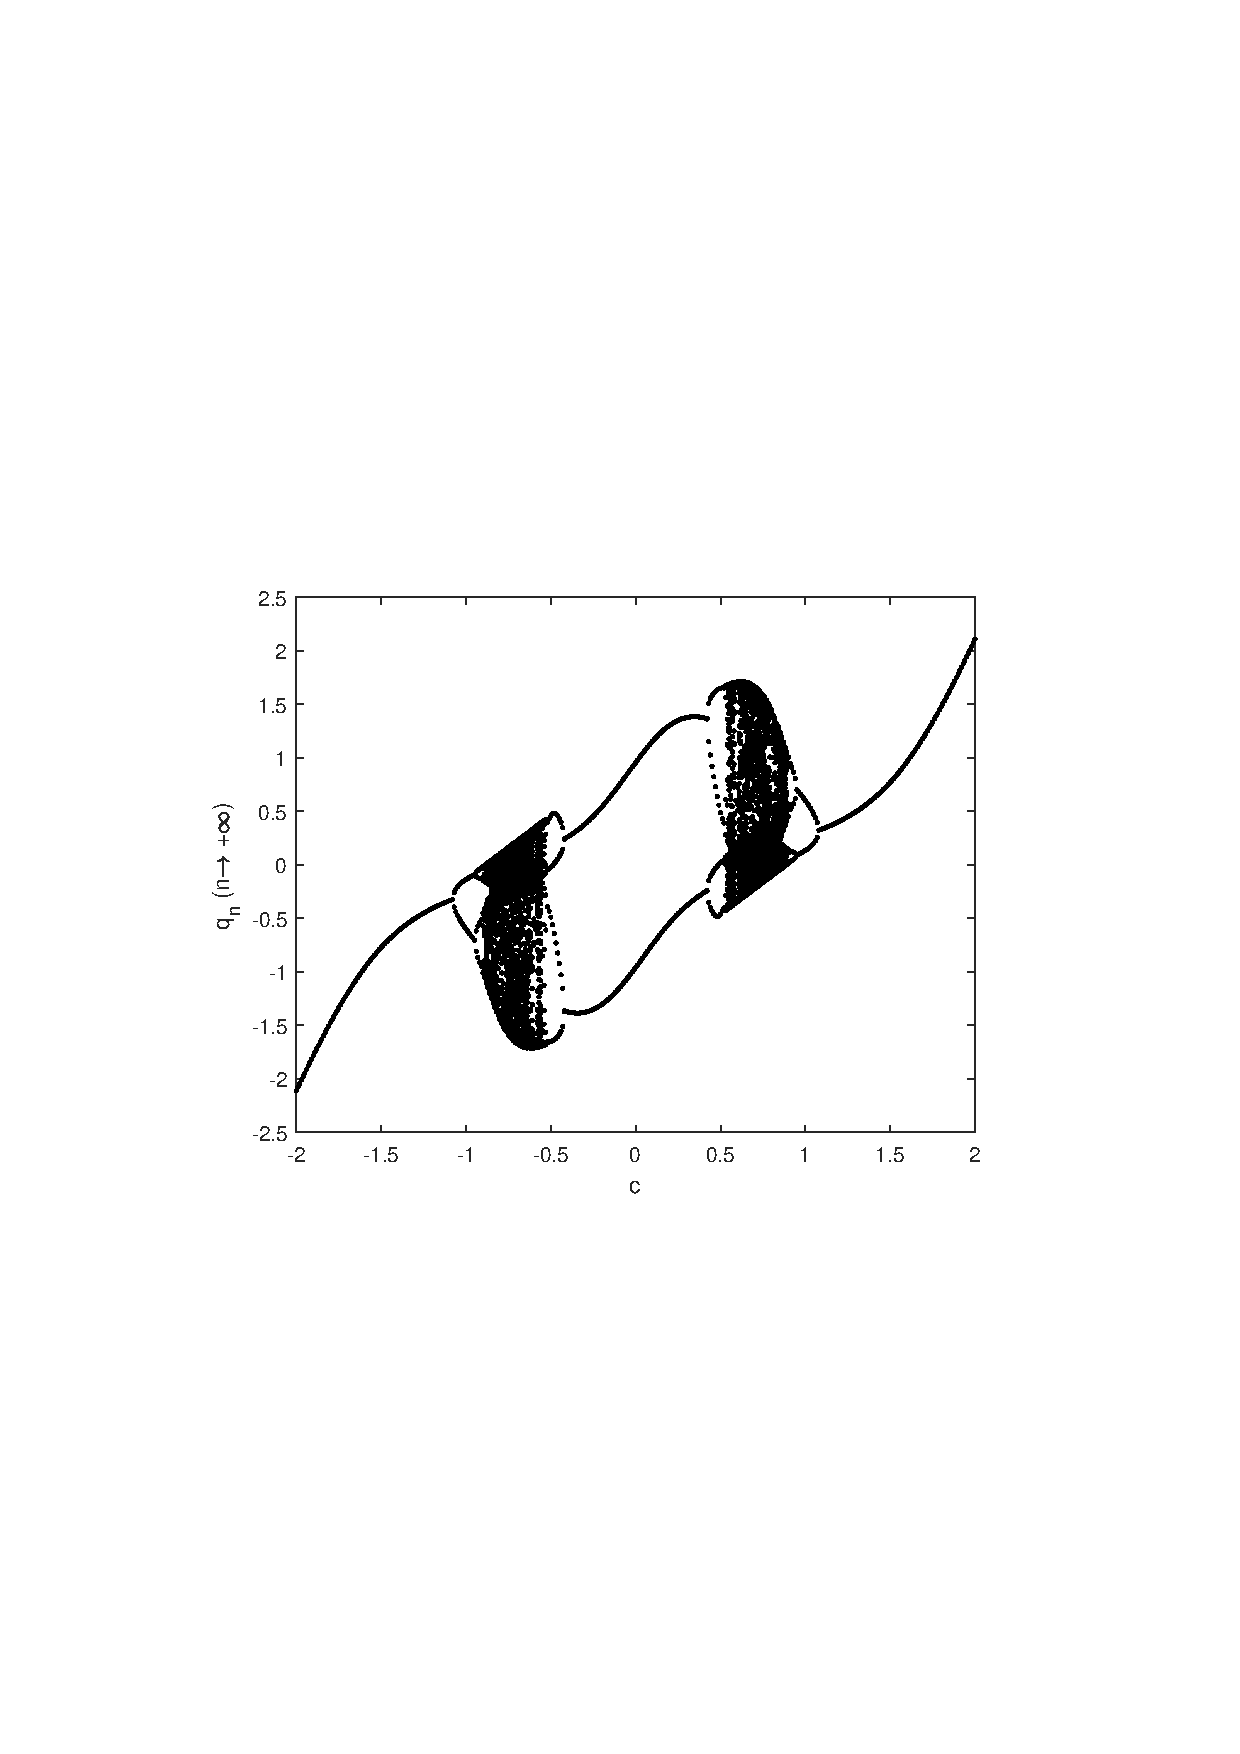
\includegraphics[width=\textwidth,trim={3.09cm 9.295cm 3.09cm 9.295cm},clip]{fig/ex8_chaos.pdf}
    \caption{期望价格$q_t$的分岔与混沌现象}
    \label{fig:ex8_chaos}
\end{figure}

\begin{table}[t]
    \centering
    \caption{前六个分岔点位置,其中$c_n$表示第$n$个分岔点。}
    \label{tab:ex8_forks}
    \begin{tabular}{c|cccccc}
        \toprule
        \(n\) & 1 & 2 & 3 & 4 & 5 & 6\tabularnewline
        \midrule
        \(c_n\) & 1.0795 & 0.9486 & 0.9071 & 0.8971 & 0.8948 &
        0.8943\tabularnewline
        \(\frac{c_n-c_{n-1}}{c_{n+1}-c_n}\) & / & 3.1542 & 4.1500 & 4.3478 &
        4.6000 & /\tabularnewline
        \bottomrule
    \end{tabular}
\end{table}

\begin{figure}[t]
    \centering
    \subfigure[第一个分岔点]{
        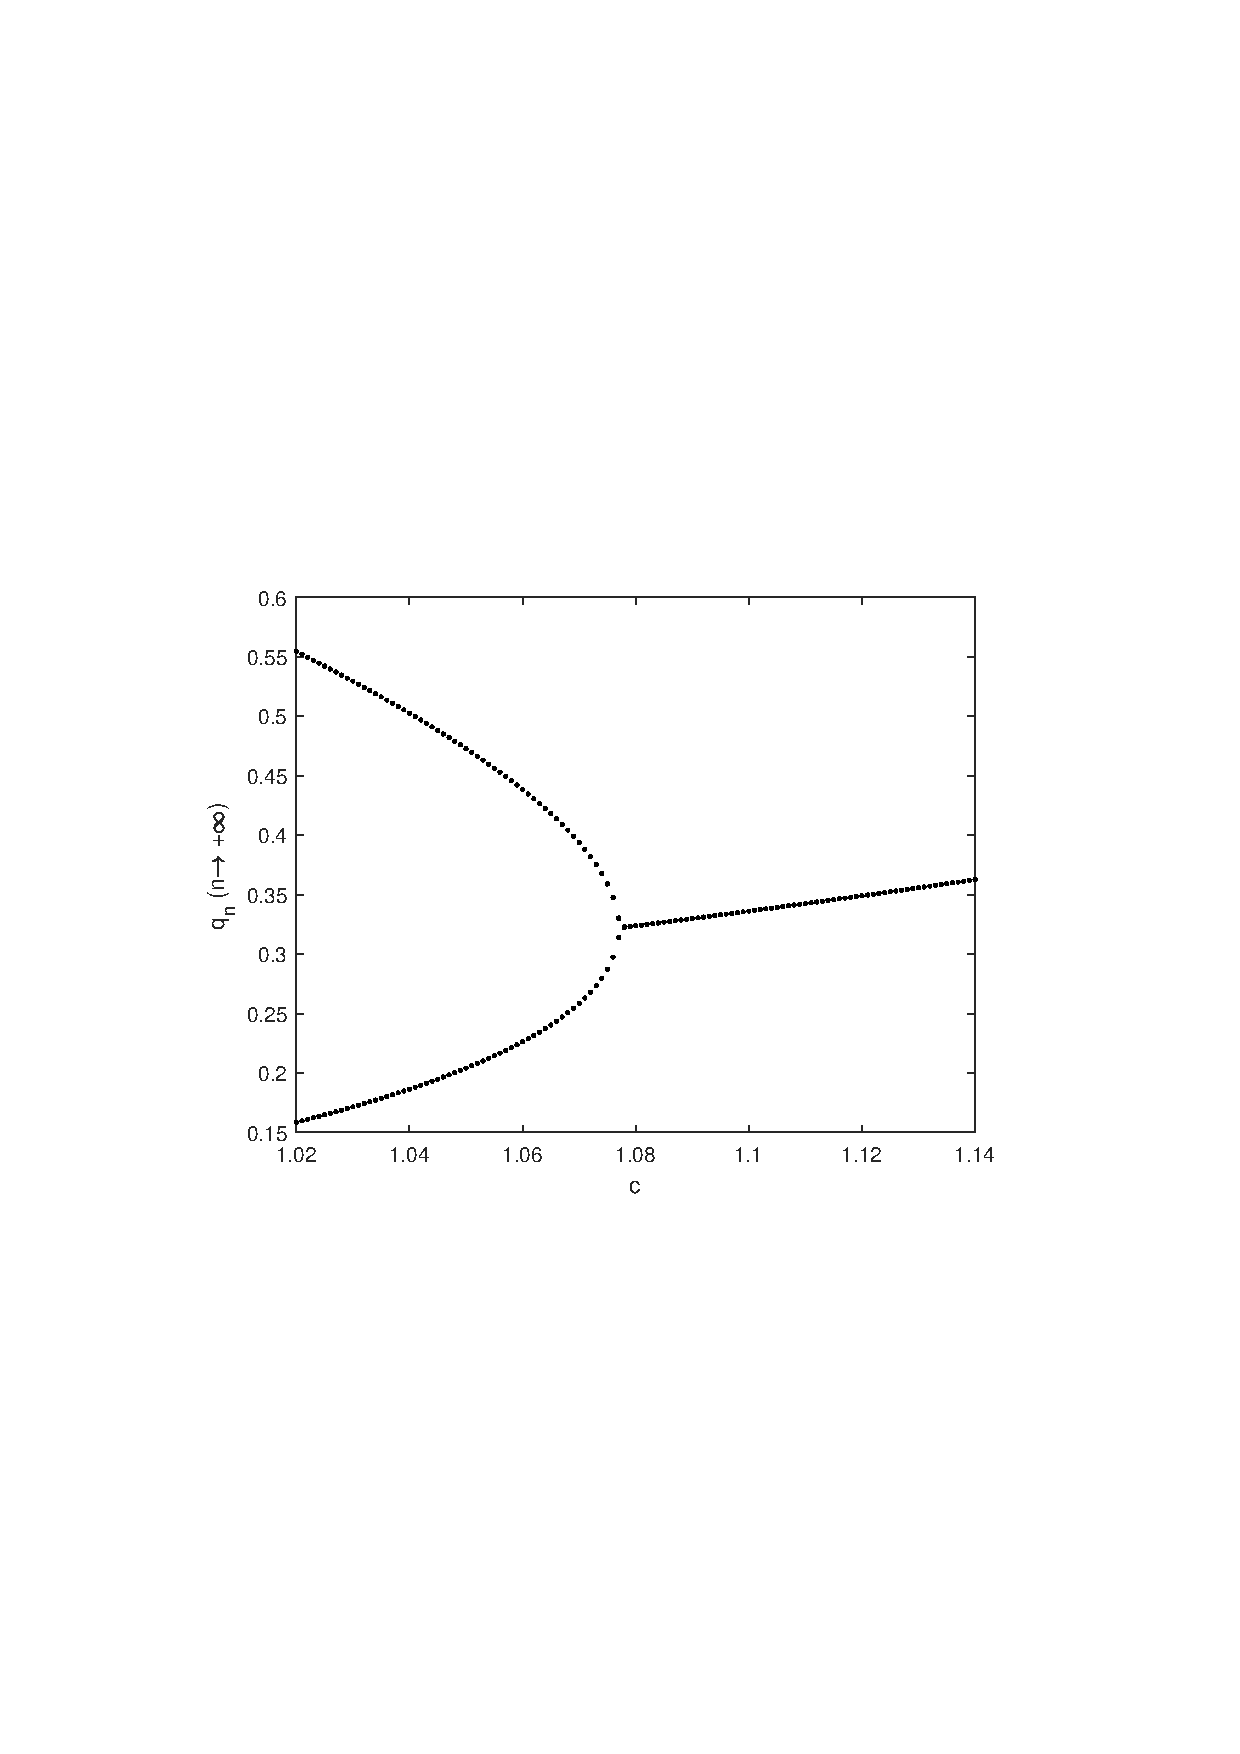
\includegraphics[width=0.47\textwidth,trim={3.09cm 9.295cm 3.09cm 9.295cm},clip]{fig/ex8_chaos_fork1.pdf}
    }
    \subfigure[第二个分岔点]{
        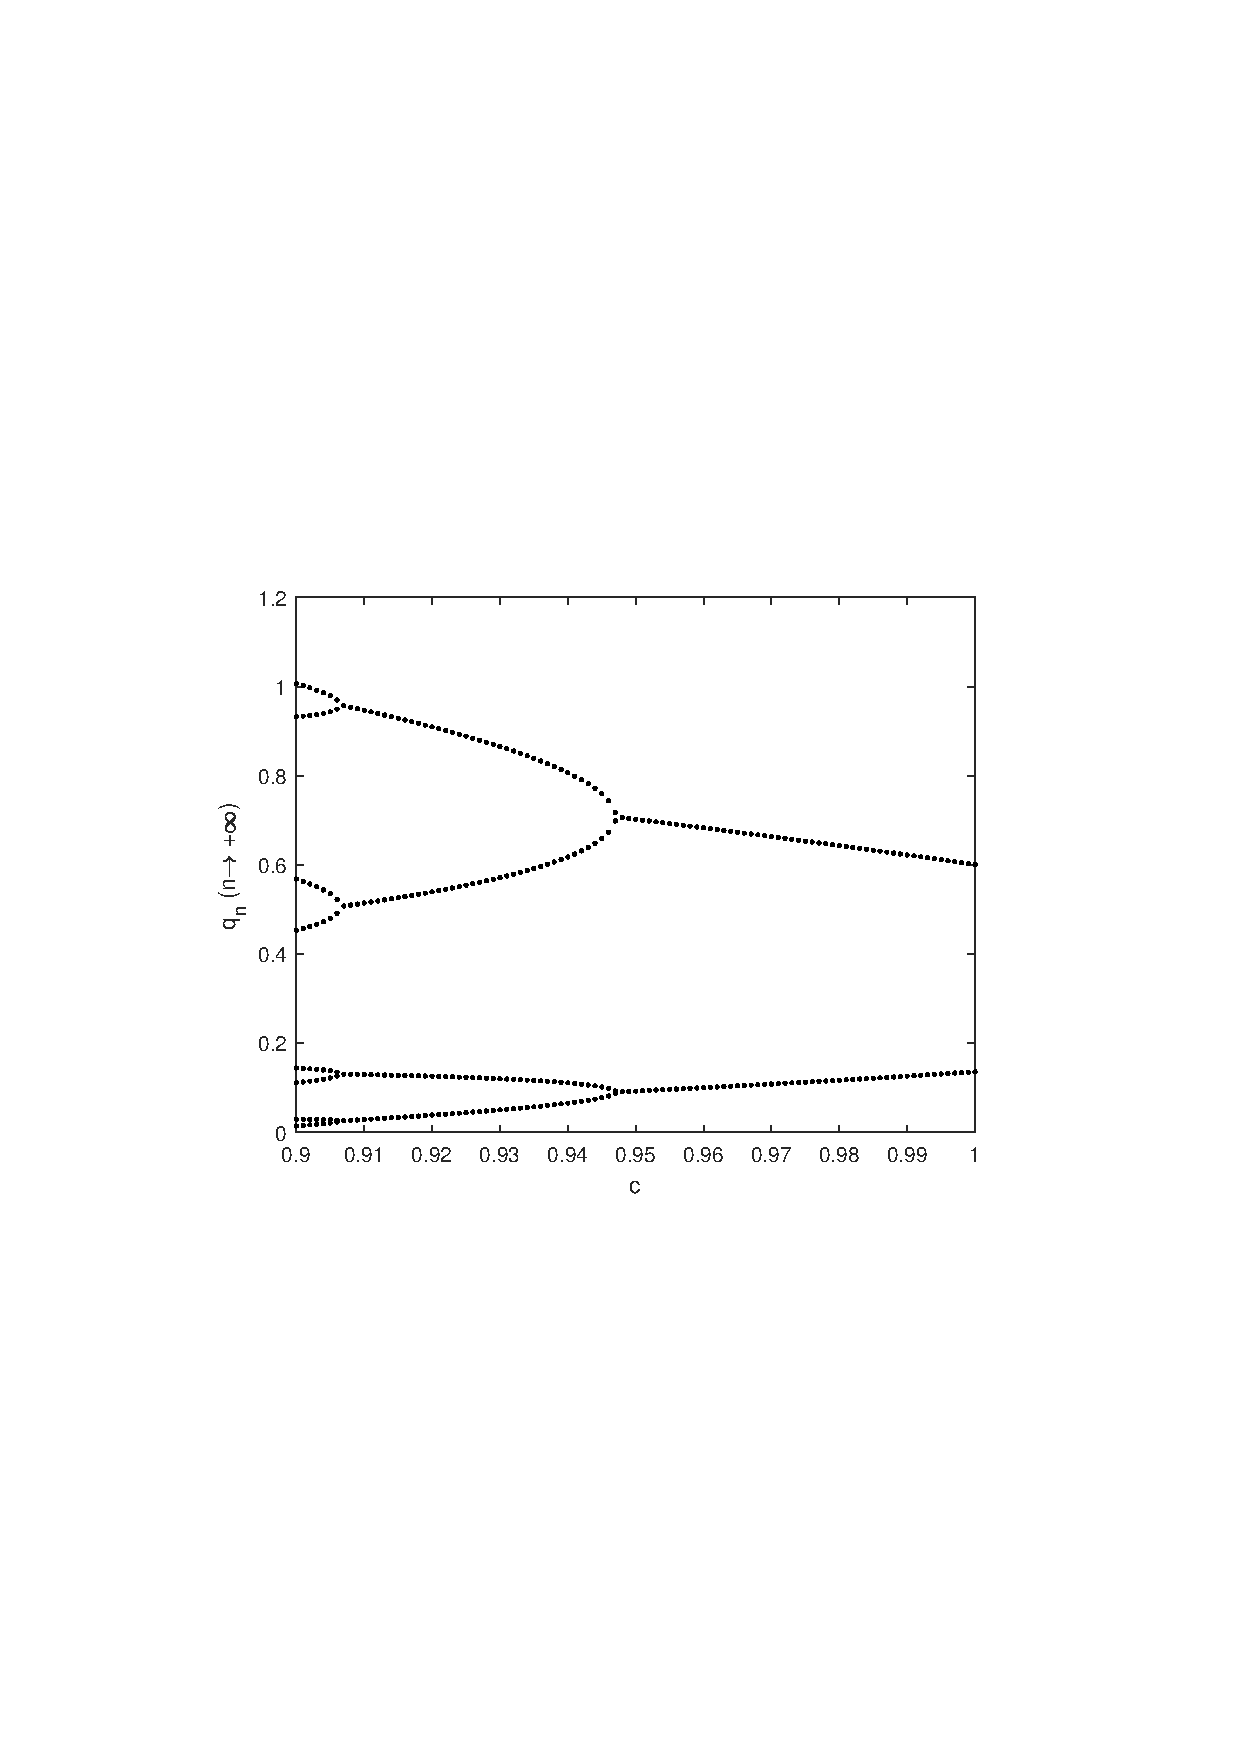
\includegraphics[width=0.47\textwidth,trim={3.09cm 9.295cm 3.09cm 9.295cm},clip]{fig/ex8_chaos_fork2.pdf}
    }
    \subfigure[第三个分岔点]{
        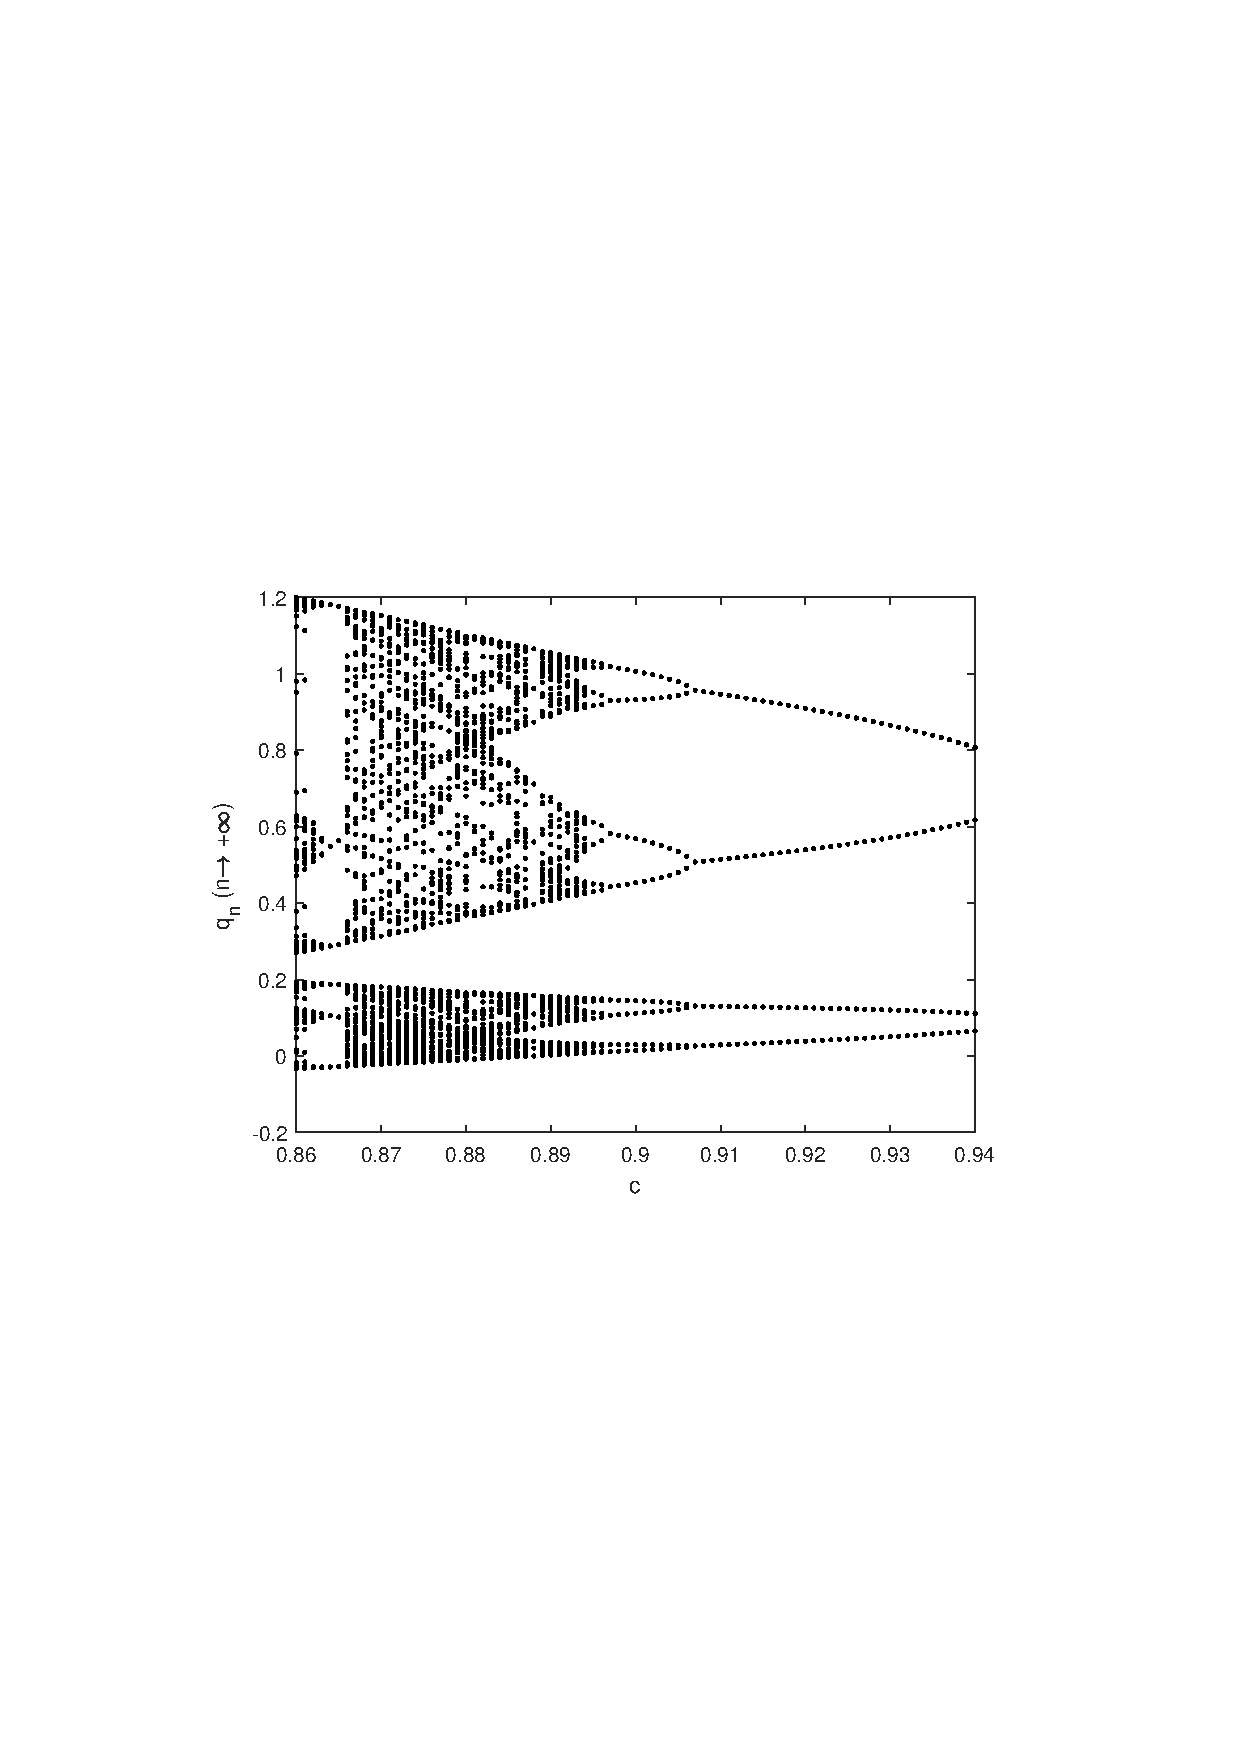
\includegraphics[width=0.47\textwidth,trim={3.09cm 9.295cm 3.09cm 9.295cm},clip]{fig/ex8_chaos_fork3.pdf}
    }
    \subfigure[第四个分岔点]{
        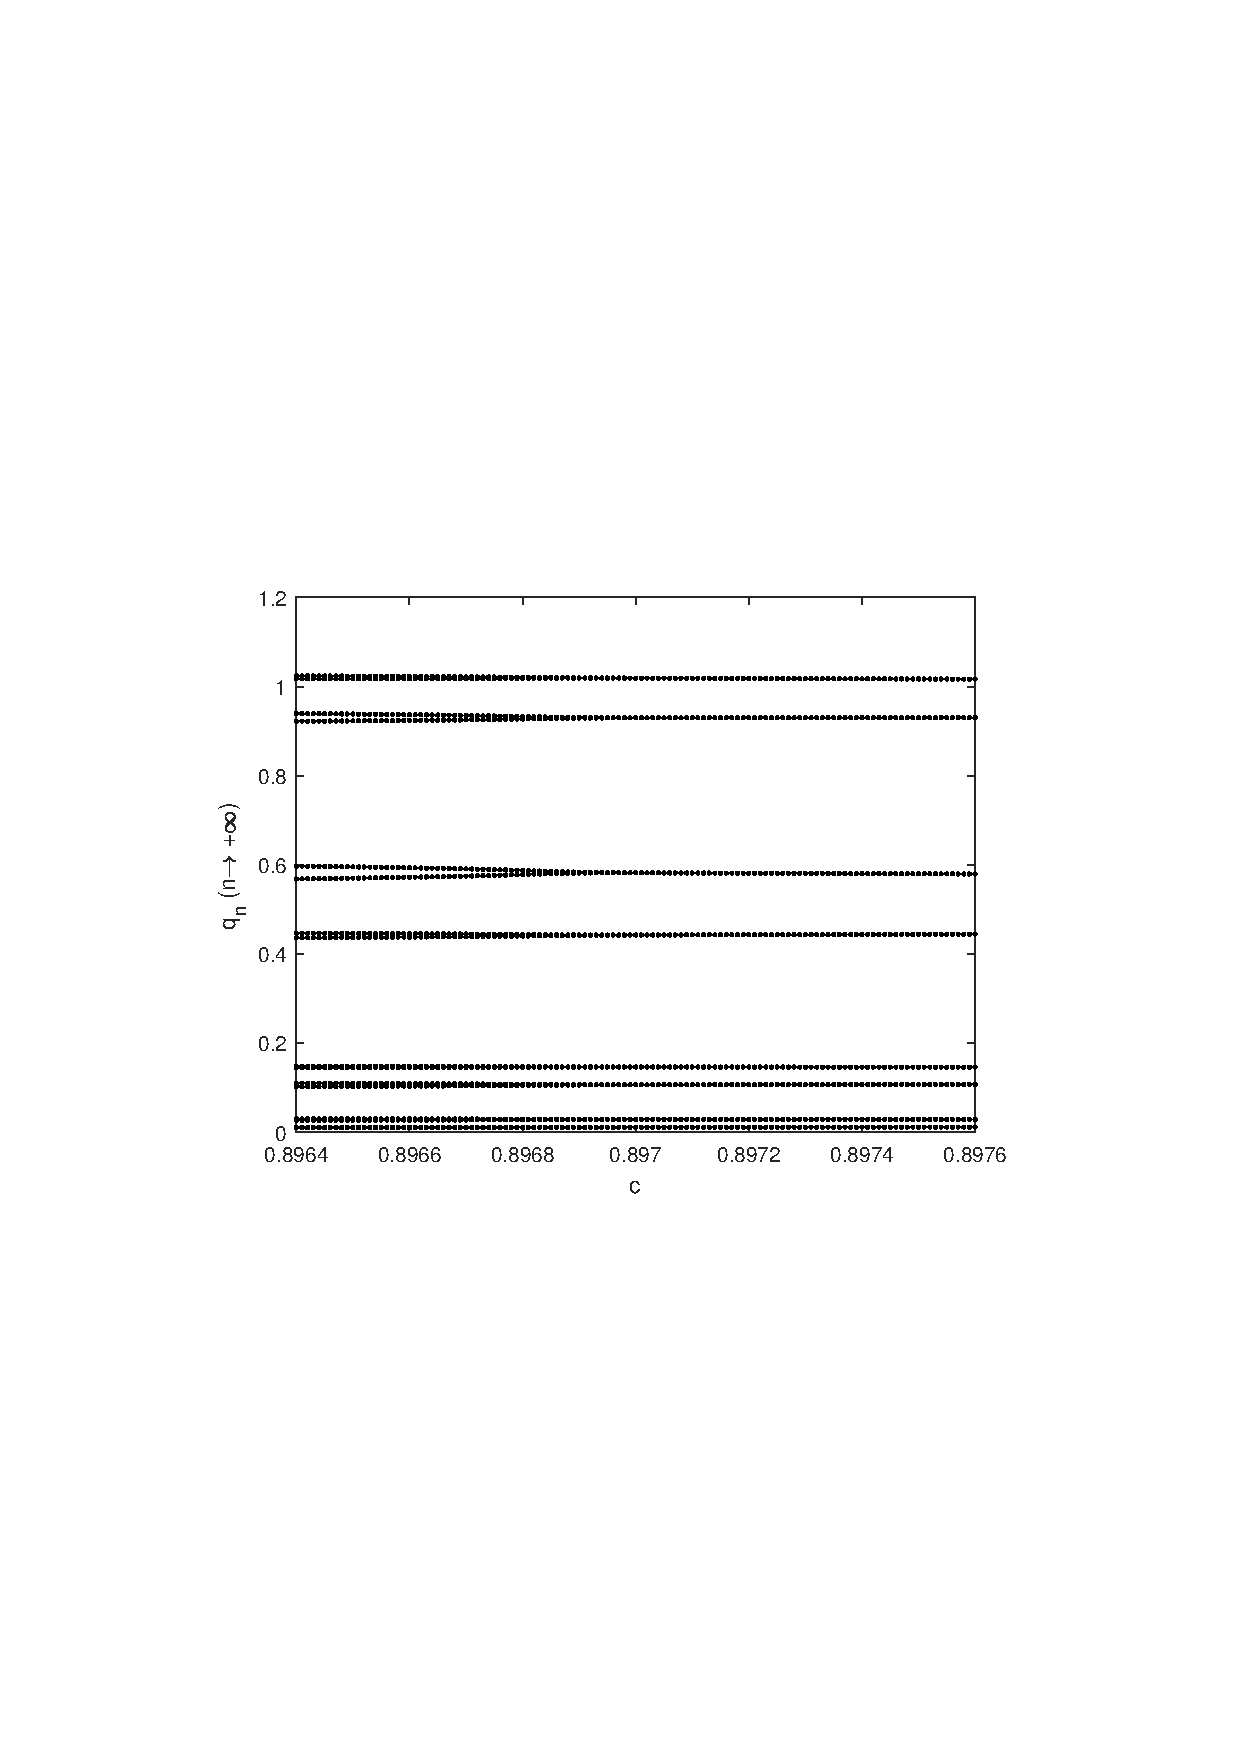
\includegraphics[width=0.47\textwidth,trim={3.09cm 9.295cm 3.09cm 9.295cm},clip]{fig/ex8_chaos_fork4.pdf}
    }
    \caption{前四个分岔点附近的图像}
    \label{fig:ex8_forks}
\end{figure}

\begin{figure}
    \centering
    \subfigure[当$c=2.0000$时的序列$q_t$图像]{
        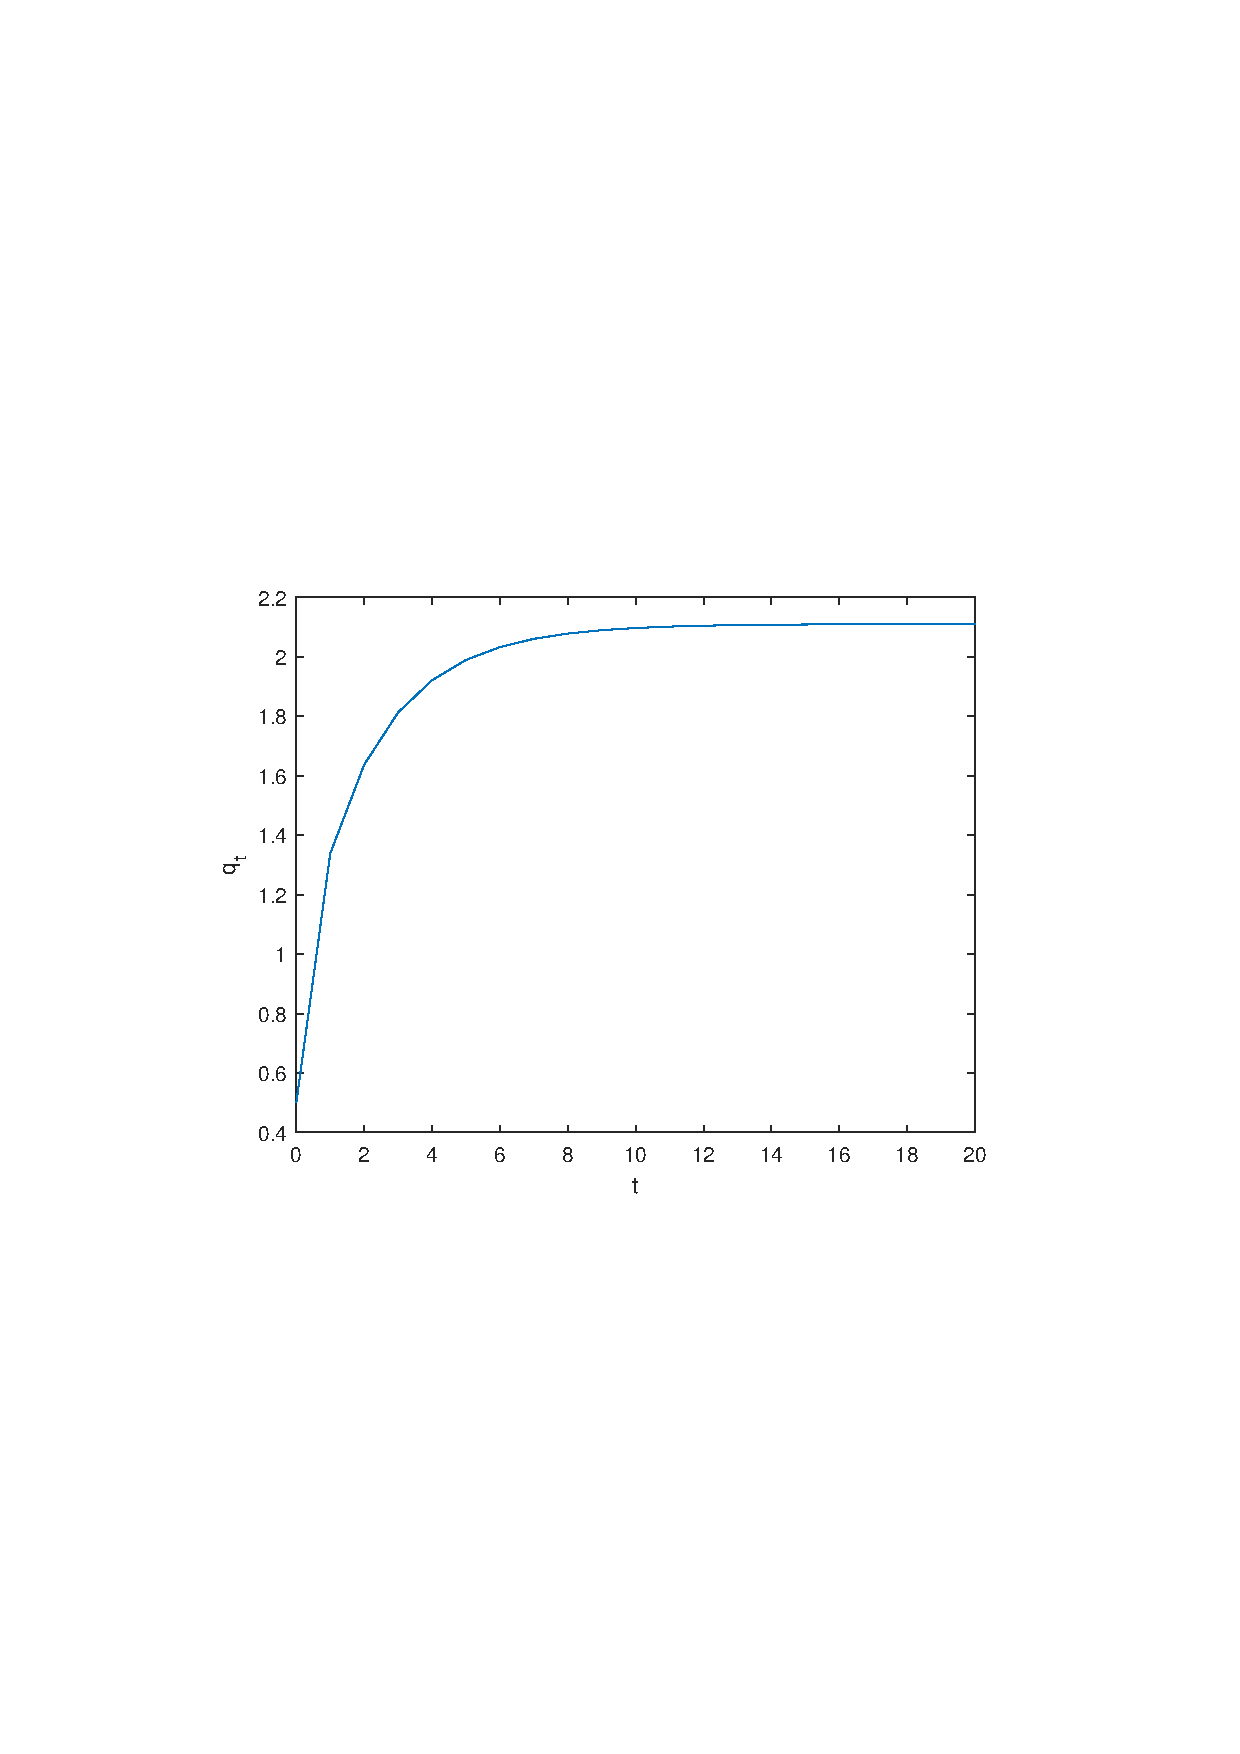
\includegraphics[width=0.47\textwidth,trim={3.09cm 9.295cm 3.09cm 9.295cm},clip]{fig/ex8_chaos_way_1.pdf}
    }
    \subfigure[当$c=1.0000$时的序列$q_t$图像]{
        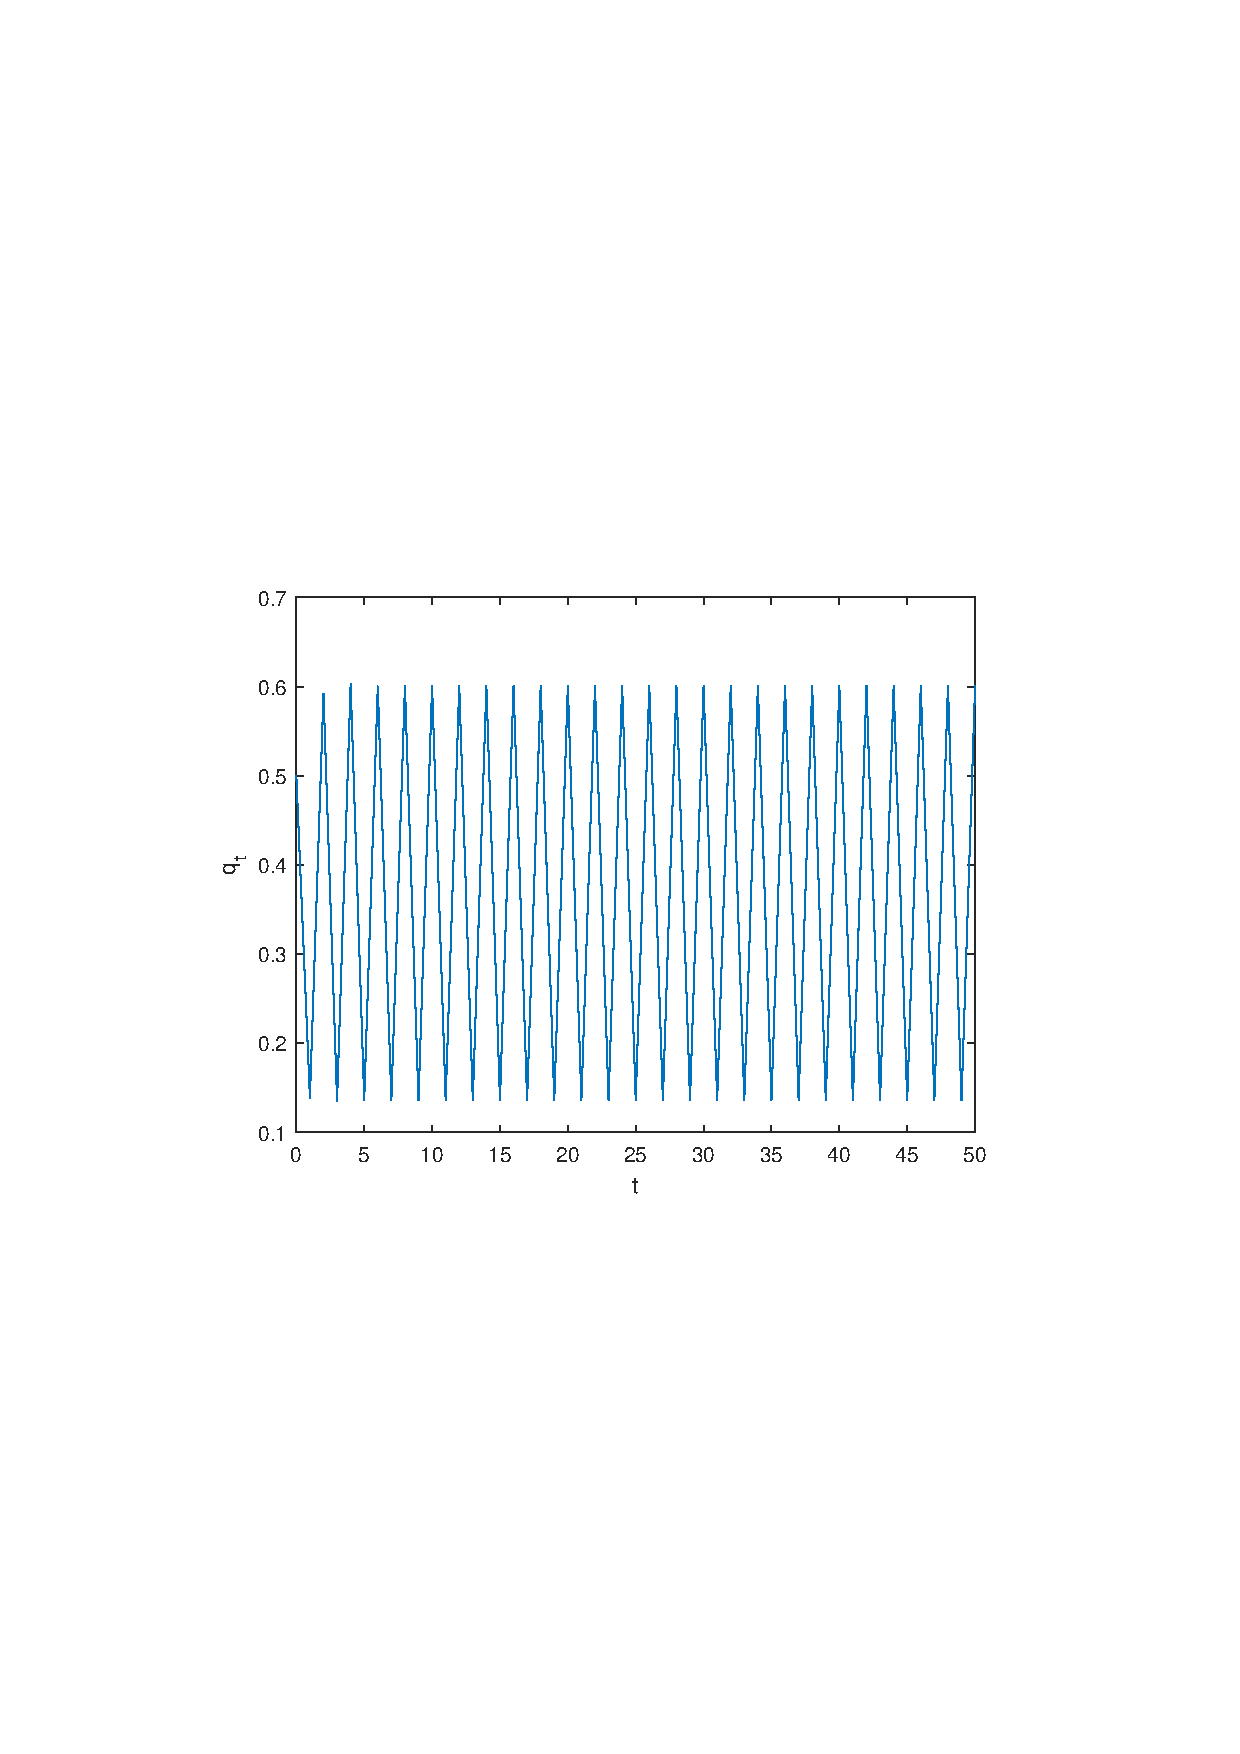
\includegraphics[width=0.47\textwidth,trim={3.09cm 9.295cm 3.09cm 9.295cm},clip]{fig/ex8_chaos_way_2.pdf}
    }
    \subfigure[当$c=0.9200$时的序列$q_t$图像]{
        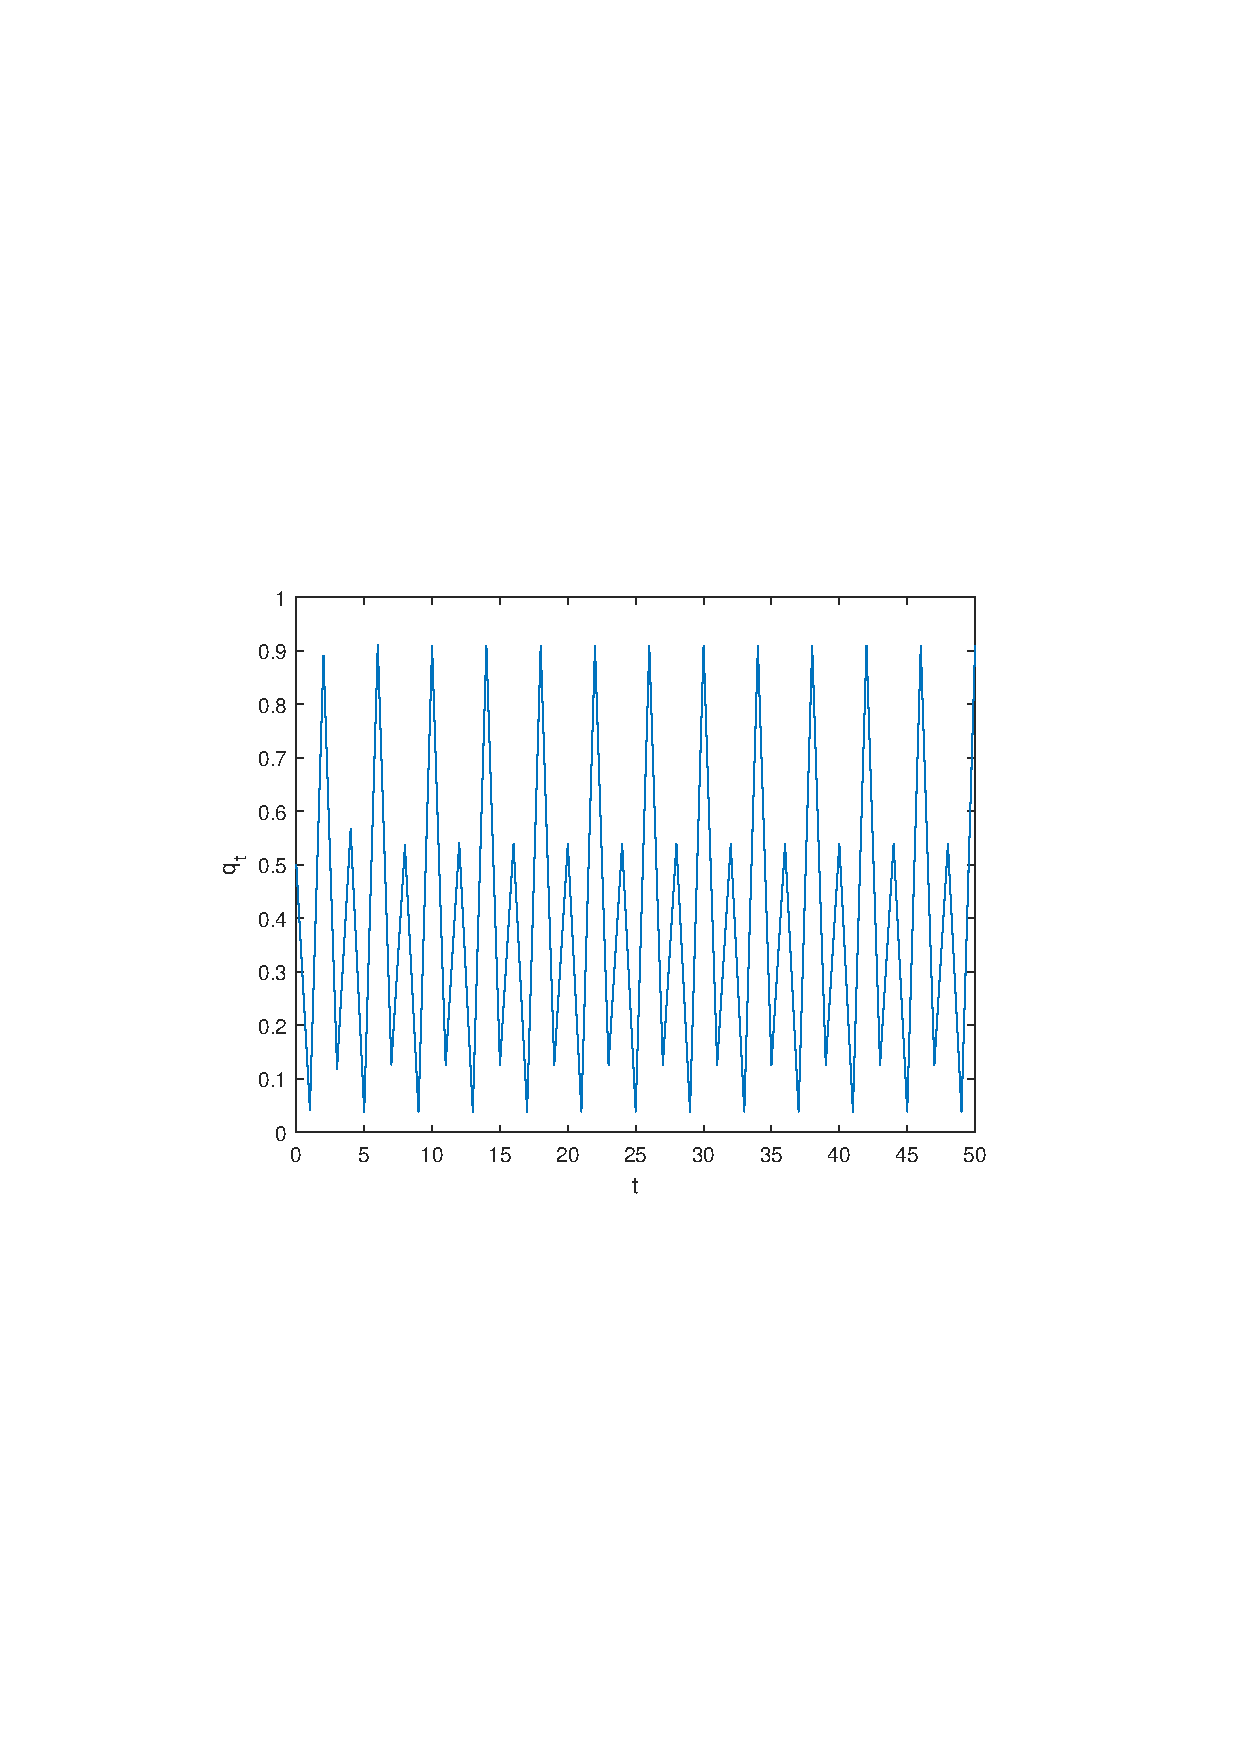
\includegraphics[width=0.47\textwidth,trim={3.09cm 9.295cm 3.09cm 9.295cm},clip]{fig/ex8_chaos_way_4.pdf}
    }
    \subfigure[当$c=0.9000$时的序列$q_t$图像]{
        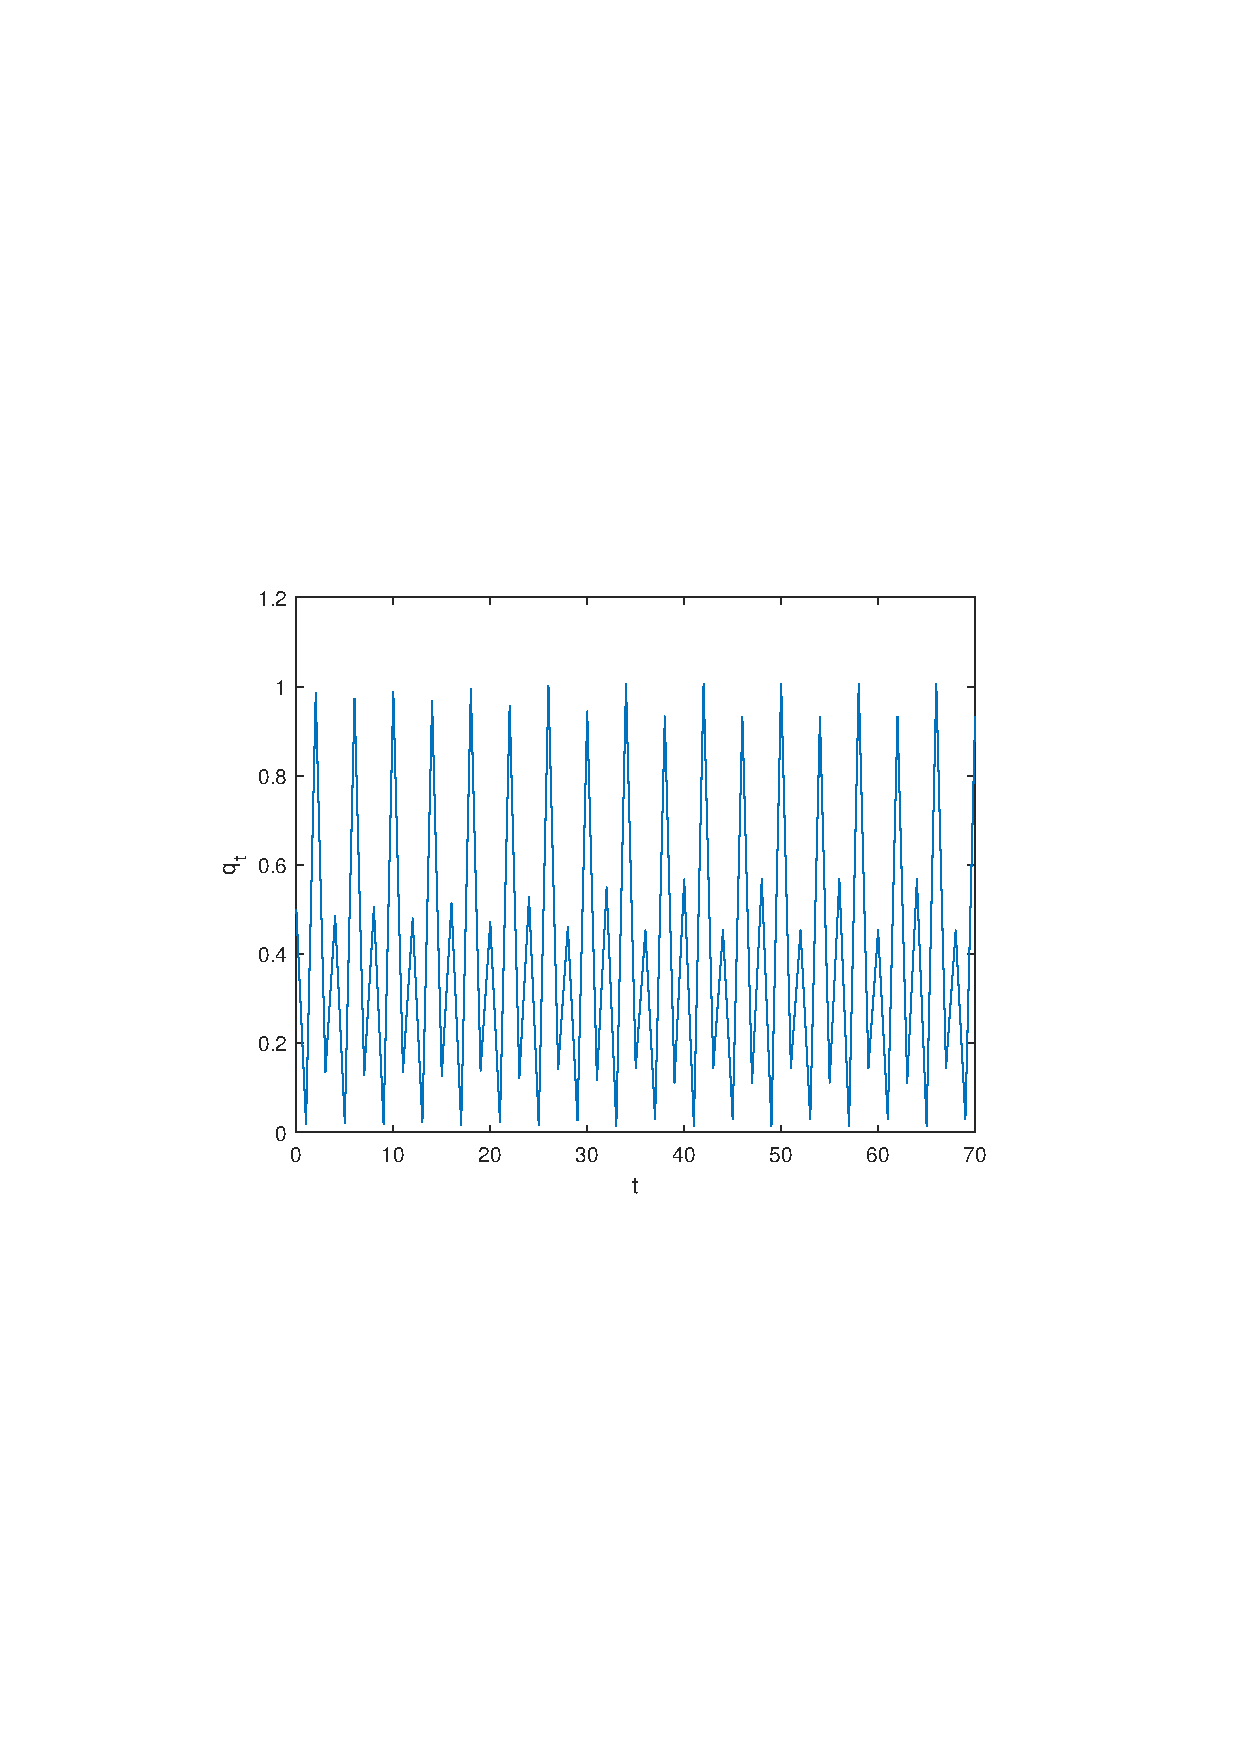
\includegraphics[width=0.47\textwidth,trim={3.09cm 9.295cm 3.09cm 9.295cm},clip]{fig/ex8_chaos_way_8.pdf}
    }
    \subfigure[当$c=0.8960$时的序列$q_t$图像]{
        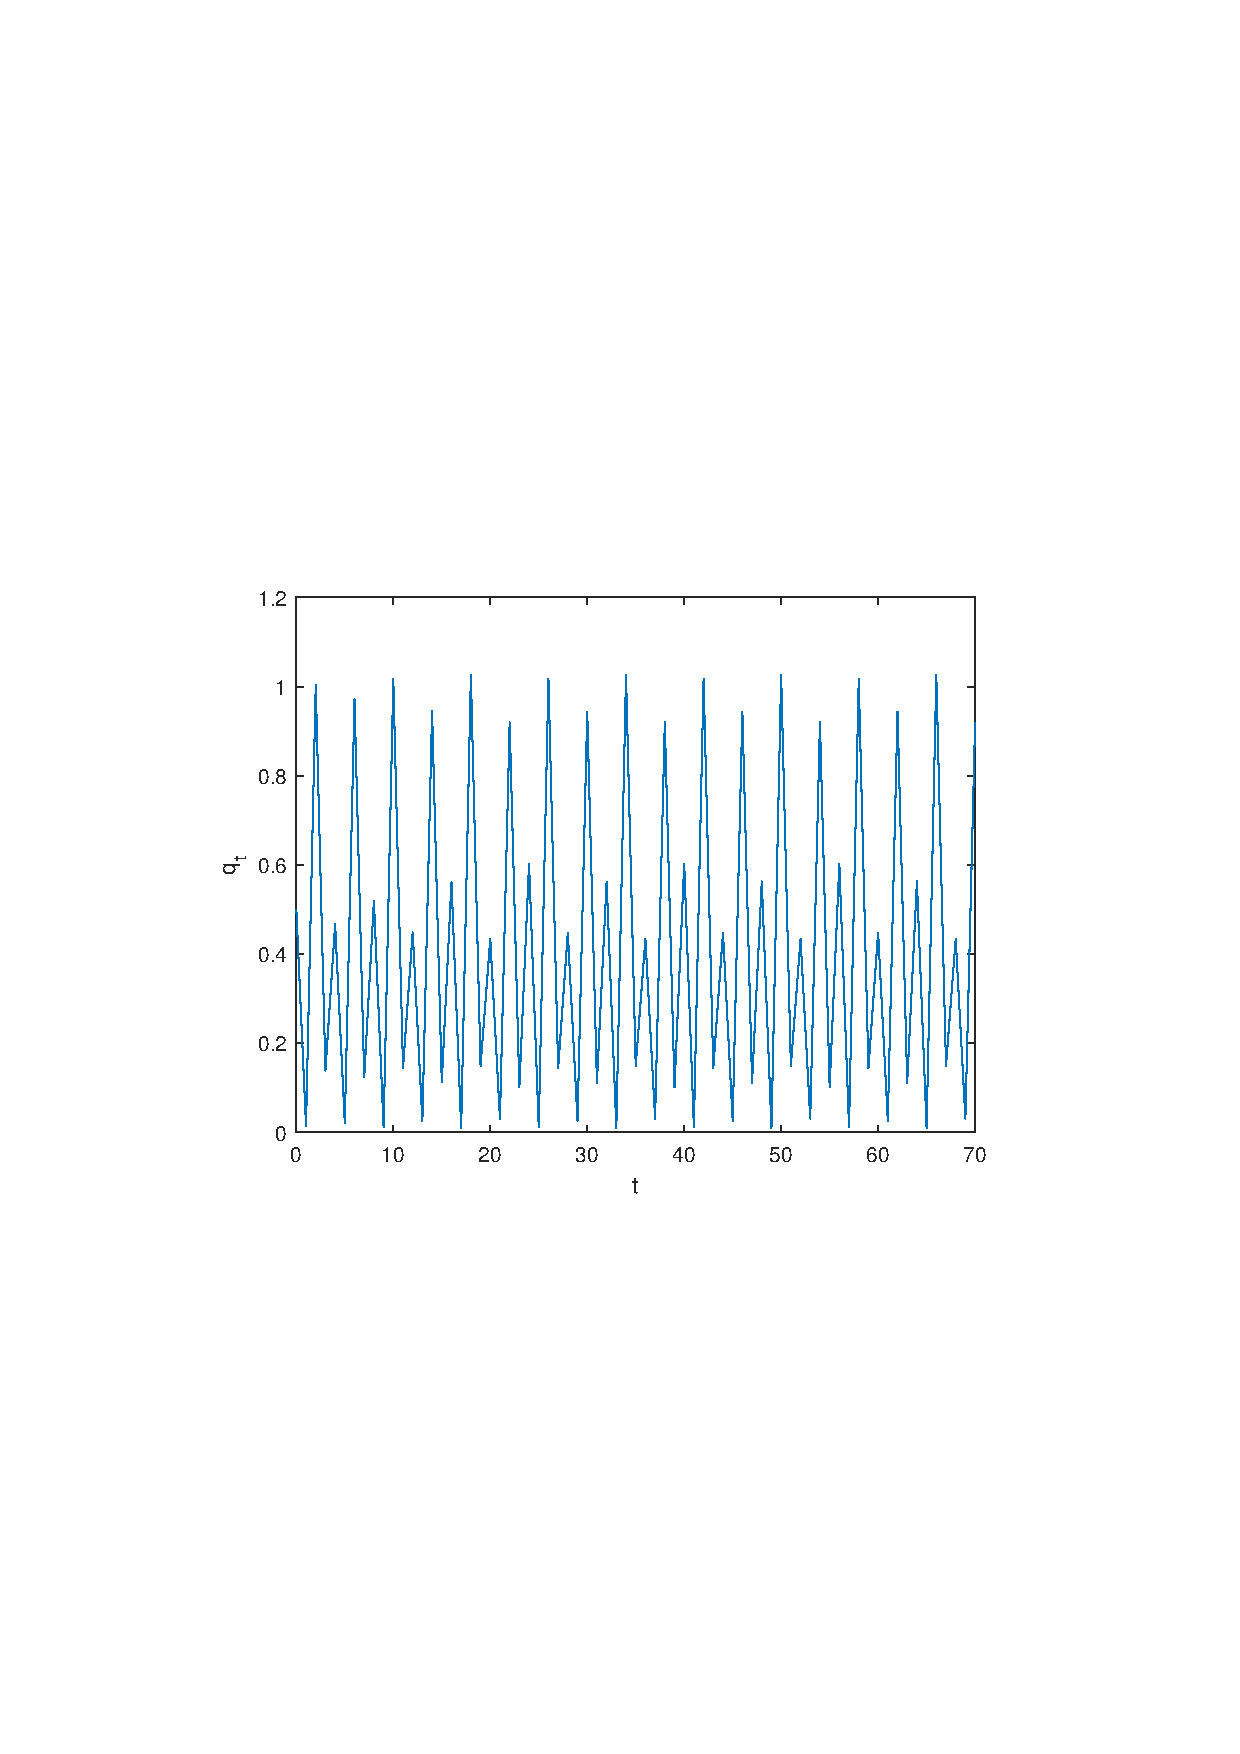
\includegraphics[width=0.47\textwidth,trim={3.09cm 9.295cm 3.09cm 9.295cm},clip]{fig/ex8_chaos_way_16.pdf}
    }
    \subfigure[当$c=0.8945$时的序列$q_t$图像]{
        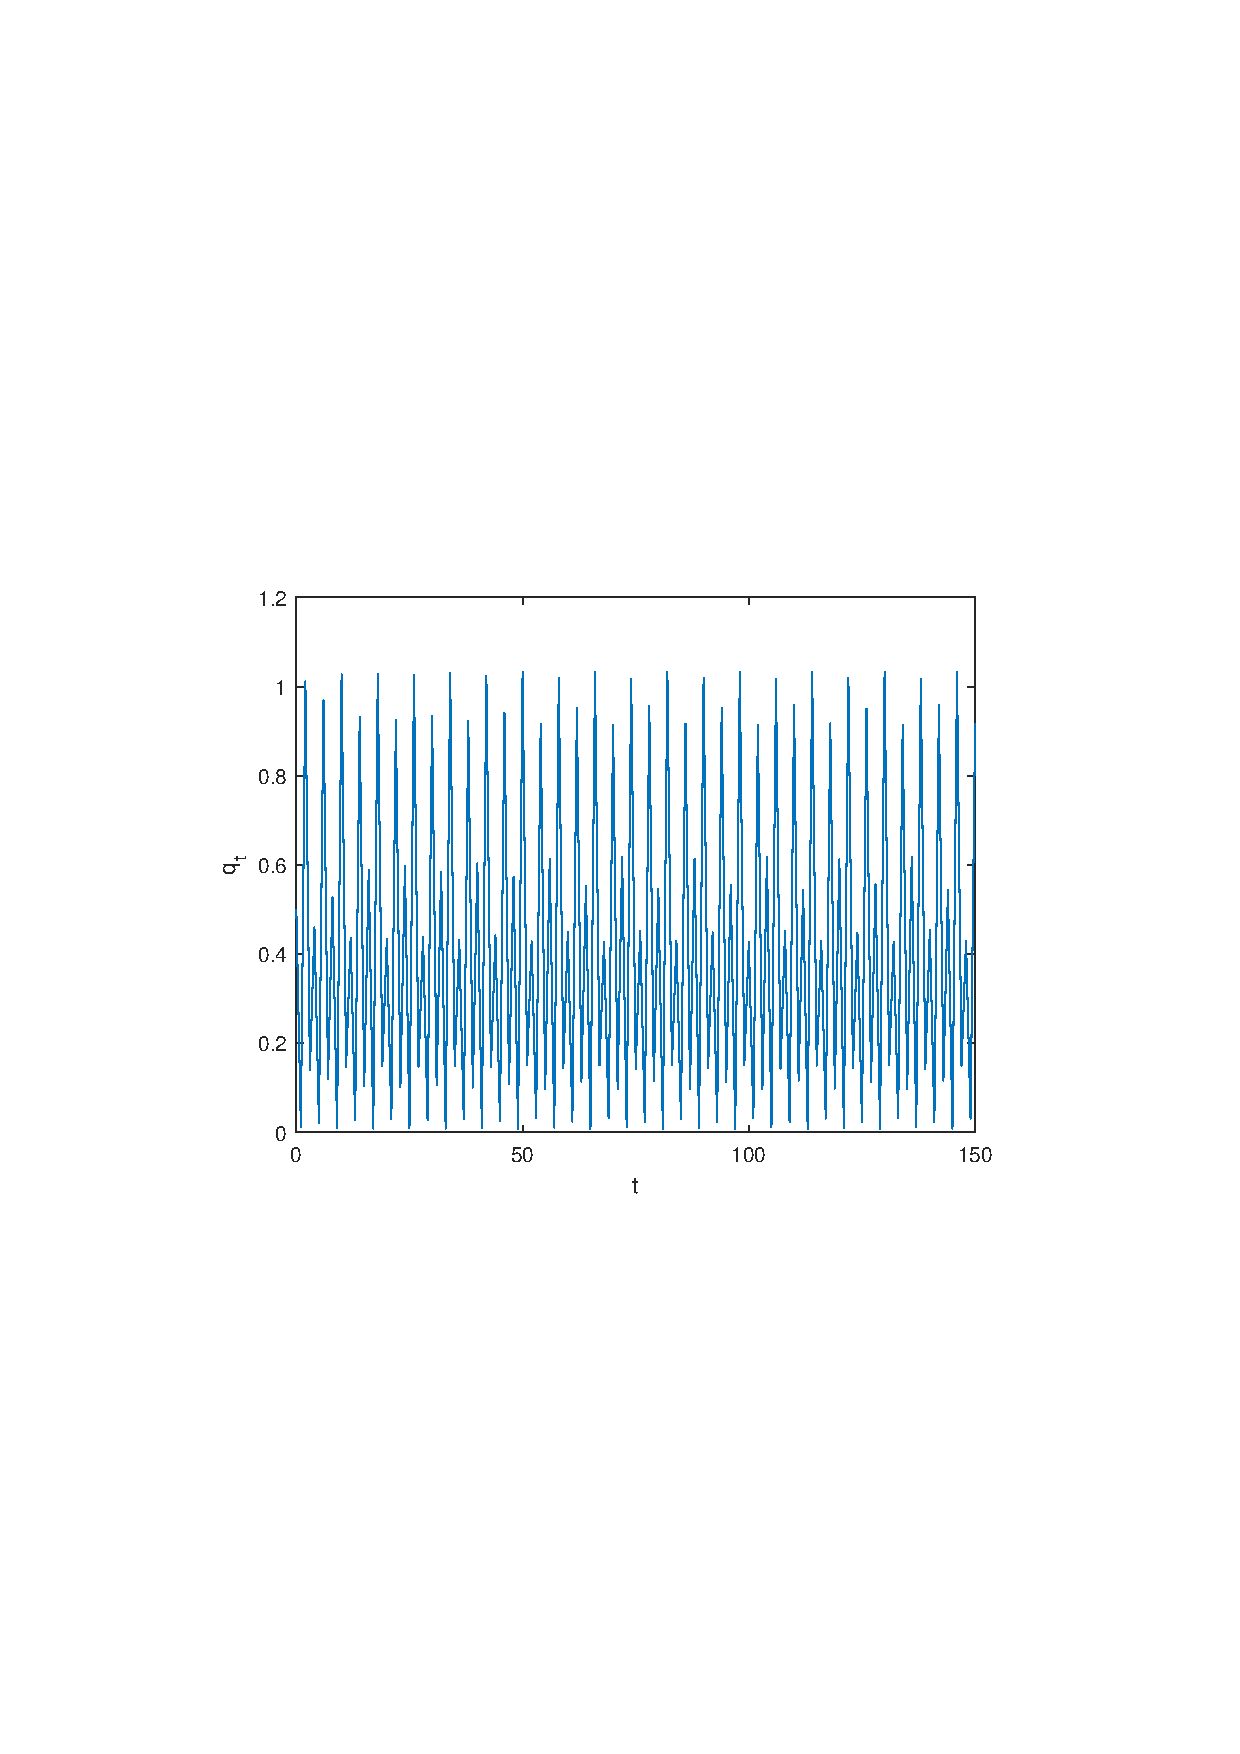
\includegraphics[width=0.47\textwidth,trim={3.09cm 9.295cm 3.09cm 9.295cm},clip]{fig/ex8_chaos_way_32.pdf}
    }
    \caption{参数$c$取不同值下的序列$q_t$图像}
    \label{fig:ex8_q_t}
\end{figure}


\subsubsection{结果分析}

从\Cref{fig:ex8_chaos}可以看出,随着参数$c$的变化,\Cref{eq:ex8_model}的序列极限出现了分岔现象,每次分岔时分岔数量增加到原来的两倍,因此分岔数呈指数增长,这样就导致了混沌现象。

从\Cref{tab:ex8_forks}可以看出,随着$n$的增长,差值比$\dfrac{c_n-c_{n-1}}{c_{n+1}-c_n}$逐渐趋近于Feigenbaum常数4.6692,大致验证了分岔点的极限规律。从这个规律中可以看出,每经过一个分岔点,相邻两个分岔点的间隔就缩小一次,也就是说,随着参数的变化,当分岔数越多,分岔增加的速度就越快,这样类似于正反馈的分岔机制也是导致混沌的一个重要原因。

从\Cref{fig:ex8_q_t}可以看出,当$c_1 < c$时,价格$q_t$收敛到一个固定的值,当$c_2 < c < c_1$时,价格$q_t$在两个定值之间来回振荡,有两个收敛的子序列,当$c_3<c<c_2$时,价格$q_t$在四个定值之间来回振荡,有四个收敛的子序列,以此类推,随着分岔数量的指数增长,$q_t$的发散程度越来越严重,出现了混沌现象。在一定程度上,$q_t$的分岔与混沌现象也反映了市场经济的周期性现象。

\subsubsection{结论}

当参数$c$在区间$[0,2]$变化时,生产方期望价格会出现分岔和混沌现象,反映了市场经济的周期性现象。

\section{收获与建议}

在本次实验中,我掌握了用MATLAB软件求解非线性方程和方程组的基本方法,并对结果进行了初步分析,用非线性方程和方程组建立了实际问题的模型,在解决实际问题的过程中,我对数学方法的原理和应用有了更深刻的理解。

希望助教能对每次的实验进行详细的解答,希望老师在未来的课堂上介绍更多数学应用的前沿知识。

\section{附录:Matlab程序代码}

\subsection{Chap6-Ex3}\label{sec:ex3_code}

\lstinputlisting[language=Matlab]{../src/ex3.m}

\subsection{Chap6-Ex6}\label{sec:ex6_code}

\lstinputlisting[language=Matlab]{../src/ex6.m}

\subsection{Chap6-Ex8}\label{sec:ex8_code}

\lstinputlisting[language=Matlab]{../src/ex8.m}

\end{document}